% !LW recipe=latexmk (XeLaTeX)
% !TeX program = xelatex
% !TeX encoding = UTF-8
\documentclass[zihao=-4,a4paper,UTF8,fontset=none]{ctexart}

% template
\usepackage{cumcm2026}
\setcitestyle{numbers}
\usepackage{xeCJK-listings}
\usepackage{booktabs}
\usepackage{graphicx}
\usepackage{float}
\setlength{\abovedisplayskip}{8pt}
\setlength{\belowdisplayskip}{8pt}
\setlength{\abovedisplayshortskip}{6pt}
\setlength{\belowdisplayshortskip}{6pt}
% set English and Number font
\setmainfont{TimesNewRoman.ttf}[
  Path=fonts/,
  BoldFont=TimesNewRomanBold.ttf,
  ItalicFont=TimesNewRomanItalic.ttf,
  BoldItalicFont=TimesNewRomanBoldItalic.ttf
]



% set Chinese font
\setCJKmainfont[
  Path=fonts/,
  BoldFont=SimHei.ttf
]{SimSun.ttc}

\setCJKfamilyfont{zhsong}[
  Path=fonts/
]{SimSun.ttc}

\setCJKfamilyfont{zhhei}[
  Path=fonts/
]{SimHei.ttf}

\setCJKmonofont[Path=fonts/,BoldFont=SimHei.ttf]{SimSun.ttc}
\newfontfamily\cumcmcodefont{DejaVuSansMono.ttf}[
  Path=fonts/,
  BoldFont=DejaVuSansMono-Bold.ttf,
  ItalicFont=DejaVuSansMono-Oblique.ttf,
  BoldItalicFont=DejaVuSansMono-BoldOblique.ttf
]

\providecommand{\songti}{}
\providecommand{\heiti}{}
\renewcommand{\songti}{\CJKfamily{zhsong}}
\renewcommand{\heiti}{\CJKfamily{zhhei}}

%标题与关键词（代码很特殊的写在document环境之前）
\title{基于联合误差场景与分布鲁棒优化的微网购电及储能调度}
\newcommand{\keywords}{\textbf{微网经济调度；储能优化；随机规划；滚动优化；非前瞻决策；分布鲁棒优化}}

\begin{document}

% 2026 电子提交版不得包含承诺书和编号专用页；第一页直接为摘要页。
\maketitle

\begin{cumcmabstract}


针对非孤岛式微网中光伏出力、负荷需求及外网电价变化引起的供需失配与购电成本不确定性，本文以 $10\,\mathrm{min}$ 为统一调度尺度，严格遵循信息非前瞻原则，按照“确定性日前调度--源荷不确定性下的随机补救--多时点预报更新下的滚动调整--源荷价联合不确定性下的分布鲁棒调度”的递进思路，建立\textbf{微网购电与储能协同优化模型}。

问题一中，在负荷、电价和光伏预测已知的条件下，建立考虑能量平衡、储能状态转移及充放电互斥等约束的\textbf{混合整数线性规划模型}。最优方案全天购电量为 $59482.70\,\mathrm{kWh}$，购电费用为 $35126.95$ 元，且无弃光发生，各项运行约束均得到满足。

问题二进一步考虑源荷预测误差，采用因果滚动预测构造\textbf{源荷联合样本外误差场景}，并建立带参数化非前瞻储能补救策略的随机优化模型。由 $5$ 倍紧急购电机制可得净负荷低估与高估的边际损失比为 $4{:}1$，对应 $80\%$ 临界分位。$2$--$12$ 月真实回放中，紧急购电量仅占实际外购电量的 $0.60\%$，但费用占比达到 $4.77\%$，表明供能不足具有显著的\textbf{非对称经济风险}。

问题三利用 $0{:}00$、$6{:}00$、$12{:}00$ 和 $18{:}00$ 的最新光伏预报及当前储能状态滚动修正后续策略，建立\textbf{四时点随机滚动调度模型}。相邻预报共同可比区间内，后三次更新使光伏预测 MAE 分别下降 $47.94\%$、$67.95\%$ 和 $31.50\%$。$334$ 个评价日回放表明，四时点策略使总费用由 $1419.63$ 万元降至 $1338.77$ 万元，\textbf{下降 $5.70\%$，紧急购电量下降 $59.62\%$}，且 $269$ 日实现费用降低，说明日内预报更新具有显著经济价值，其中 $6{:}00$ 和 $12{:}00$ 更新作用最为明显。

问题四进一步考虑未来实时电价不可提前获知，基于历史信息滚动预测电价，并利用\textbf{价格--净负荷联合样本外误差}构造场景及 Wasserstein 模糊集，分别建立波动电价下的日前与四时点\textbf{分布鲁棒调度模型}。真实回放中，四时点策略较日前策略使总结算费用降低 $2.03\%$，紧急购电量和紧急购电费用分别降低 $33.30\%$ 和 $33.18\%$，且 $334$ 个运行日中有 $230$ 日费用更低。结果表明，所建模型能够有效利用逐步到达的预测信息降低高倍补购风险，并兼顾\textbf{调度经济性、供能安全性与运行可行性}。





\cumcmkeywords{\keywords}
\end{cumcmabstract}

\section{问题重述}
\subsection{问题背景}
在微网运行中，光伏出力与小区负荷随时间变化，二者在峰谷时段往往难以完全匹配，容易造成电能富余或供电不足。储能可以通过跨时段充放电调节供需，但受到容量、功率和效率等约束。因此，如何根据负荷、光伏和电价变化合理安排外网购电与储能运行，在满足用电需求的同时尽可能降低购电成本尤为重要。

\subsection{问题要求}

本题围绕非孤岛式微网中外网购电、光伏发电与储能运行的协同调度展开。
四个问题在统一的源--荷--储运行框架下逐步增加现实因素：
由确定条件下的日前调度，依次扩展到源荷变化下的紧急补购、
多时点光伏预报更新下的日内调整，以及实时波动电价下的综合调度。

\textbf{问题一：}
在不同日期采用相同的日内电价和小区负荷曲线、且当日光伏预测功率已知的条件下，
于每天 $0{:}00$ 制定全天计划购电策略。
要求微网供能满足小区负荷，并满足储能容量、充放电功率、效率以及
日初与日末储电量相等等运行约束，在此基础上确定计划购电量和储能充放电方案，
使全天购电费用尽可能低。

\textbf{问题二：}
在问题一基础上，小区负荷和光伏实际发电功率随日期和时段变化，
每天仍需在 $0{:}00$ 制定当日计划购电策略。
若实际供能不足，缺口部分需按交易时刻正常电价的 $5$ 倍紧急购电，
其余购电费用仍按计划购电量计算。
据此制定相应的计划购电、储能运行和紧急购电策略。

\textbf{问题三：}
在问题二基础上，每天 $0{:}00$、$6{:}00$、$12{:}00$ 和
$18{:}00$ 可获得未来 $24\,\mathrm h$ 的光伏发电功率预报。
根据 $0{:}00$ 预报制定全天计划，并可依据其余时点的新预报调整后续购电策略；
计划购电量高于调整购电量的部分按交易电价的 $50\%$ 计违约费用，
调整购电量高于计划购电量的部分按交易电价的 $1.5$ 倍计费，
同时仍需考虑供能不足产生的紧急购电。
据此建立日内调整策略，并分析是否有必要利用后续预报修正原计划。

\textbf{问题四：}
进一步考虑外网电价随日期和时段实时波动。
在问题二和问题三原有源荷变化及光伏预报更新条件下，
引入波动电价重新制定相应的购电与储能调度策略，
并分别给出波动电价下问题二和问题三的计算结果。




\section{模型假设与符号说明}

\subsection{模型假设}
\noindent 1) 各决策时点仅使用当时已经获得的历史信息与题目规定的预报信息，不提前使用尚未实现的真实负荷、光伏功率及实时电价。

\noindent 2) 题目未规定微网向外网售电，故不考虑反向售电；负荷及储能无法消纳的剩余光伏允许弃用，且不产生收益。

\noindent 3) 储能充、放电量均按微网母线侧计量，将题设 $90\%$ 的充放电效率解释为充电效率和放电效率均为 $0.9$；忽略自放电、寿命衰减及线路损耗。

\noindent 4) 对问题三及问题四中的多次购电调整，按各时段最终生效购电量相对当日 $0{:}00$ 原计划进行一次结算，不重复计算中间调整费用。

\subsection{通用符号说明}

\begin{center}
\renewcommand{\arraystretch}{1.30}
\setlength{\tabcolsep}{8pt}
\begin{tabularx}{0.92\textwidth}{
    >{\centering\arraybackslash}p{0.20\textwidth}
    >{\centering\arraybackslash}X
}
    \toprule
    符号 & 符号含义及说明 \\
    \midrule

    $d$
    & 日期索引 \\

    $t$
    & 单个自然日内的 $10\,\mathrm{min}$ 时段索引 \\

    $\tau$
    & 滚动优化窗口内的相对时段索引 \\

    $k$
    & 日内预报与决策节点 \\

    $s$
    & 随机场景编号 \\

    $p$
    & 外网交易电价，单位为元/kWh \\

    $E$
    & 储能设备的储电量，单位为 kWh \\

    $\eta_c,\eta_d$
    & 储能充电效率和放电效率 \\

    $E_{\min},E_{\max}$
    & 储能设备允许的最小、最大储电量，单位为 kWh \\

    $Q_{\max}$
    & 单个调度时段允许的最大充电量或放电量，单位为 kWh \\

    $n$
    & 净负荷电量，单位为 kWh \\

    $\pi_s$
    & 随机场景 $s$ 的概率 \\

    $e^{L},e^{PV},e^{N}$
    & 负荷、光伏功率及净负荷的样本外预测误差 \\

    \bottomrule
\end{tabularx}
\end{center}

\subsection{数据统一口径}
为保持各问在时间尺度、时段归属和计量单位上的一致性，
本文统一采用 $10\,\mathrm{min}$ 作为调度与运行分析的基本时间步长，记
\begin{equation}
    \Delta t=\frac{1}{6}\,\mathrm h,
    \qquad
    t=1,2,\ldots,144.
\end{equation}
其中，$t$ 表示单个自然日内的时段索引；
跨日滚动优化仍保持相同时间步长，并按时间顺序延伸索引。

对于 $10\,\mathrm{min}$ 时序数据，统一采用时段右端点进行标记。
例如，$00{:}10$ 对应区间 $[00{:}00,00{:}10)$；
$0{:}00+1$ 表示次日 $0{:}00$，即当日 $24{:}00$，
对应区间 $[23{:}50,24{:}00)$。
在按日统计、历史信息划分及滚动回测中，
该时段仍归属于原自然日。

小区负荷与光伏发电等源荷数据以功率 $\mathrm{kW}$ 表示。
预测、误差分析及其他统计环节保留功率单位；
进入调度模型时，按
\begin{equation}
    Q=P\Delta t
\end{equation}
转换为相应时段电量。
计划购电量、调整购电量、紧急购电量、
储能充放电量及储电量均以 $\mathrm{kWh}$ 计，
电价单位统一为元/kWh。

下文不再重复上述时间、索引和单位定义，
仅说明各附件特有的数据重构、时间对齐及信息处理步骤。


\section{问题一的模型建立与求解}

\subsection{问题分析}

问题一中，日内电价、小区负荷和光伏预测功率在决策时均作为已知参数，
因此本问属于确定条件下的日前经济调度问题，无需进一步刻画预测误差及随机性。
各时段的供需平衡可由外网购电、光伏发电与储能充放电共同协调，
而储电量状态又将相邻时段的决策相互耦合，
使购电与储能运行不能按单个时段独立优化。
考虑到购电成本、能量平衡、储能状态转移及运行边界均可线性表示，
同时充、放电互斥关系需要引入 $0$--$1$ 状态变量，
本文建立源--荷--储协同日前调度的混合整数线性规划模型（MILP）。

\subsection{基于 MILP 的微网源--荷--储协同调度模型} 设第 $t$ 个调度时段的外网购电量、母线侧储能充电量、储能向母线侧输出的放电量及弃光量分别为 $G_t$、$C_t$、$D_t$、$W_t$，时段末储电量为 $E_t$，并引入二元变量 $u_t$ 刻画充、放电互斥关系。 鉴于题目未规定微网向外网反向售电的交易机制，本文假定不考虑售电，并以 $W_t$ 表示未被利用的光伏电量。 以全天外网购电费用最小为目标，有 \begin{equation} \min J=\sum_{t=1}^{144} p_tG_t , \label{eq:q1_objective} \end{equation} 其中，$p_t$ 为第 $t$ 个时段的外网电价，单位为元/kWh。各时段母线侧满足能量守恒： \begin{equation} G_t+(S_t-W_t)+D_t=L_t+C_t, \qquad t=1,\ldots,144 . \label{eq:q1_balance} \end{equation} 其中，$S_t-W_t$ 为实际参与微网调度的光伏电量。式~\eqref{eq:q1_balance} 统一刻画了外网、光伏、负荷与储能之间的电量流动关系。 储能通过电量状态将相邻调度时段耦合。按照前述母线侧充、放电量定义， 第 $t$ 个时段末的储电量满足 \begin{equation} E_t = E_{t-1} +\eta_c C_t -\frac{D_t}{\eta_d}, \qquad t=1,\ldots,144 . \label{eq:q1_storage} \end{equation} 其中，$\eta_c$ 和 $\eta_d$ 分别为充电效率和放电效率。 本文主模型将题设“充放电效率为 $90\%$”解释为充、放电单程效率均为 $0.9$， 即 $\eta_c=\eta_d=0.9$。 在该计量口径下，母线侧输入 $C_t$ 后实际存入电池的能量为 $\eta_c C_t$， 而储能向母线输出 $D_t$ 时需消耗 $D_t/\eta_d$ 的内部电量。 针对效率口径可能存在的解释差异，后文进一步进行敏感性检验。 根据储电量安全运行范围、最大充放电能力以及充、放电互斥要求， 对 $t=1,\ldots,144$ 有 \begin{equation} \left\{ \begin{aligned} &1200\le E_t\le10800,\\ &0\le C_t\le Q_{\max}u_t,\\ &0\le D_t\le Q_{\max}(1-u_t),\\ &0\le W_t\le S_t,\\ &G_t\ge0,\\ &u_t\in\{0,1\}. \end{aligned} \right. \label{eq:q1_constraints} \end{equation} 其中， \[ Q_{\max} = P_{\max}\Delta t = \frac{5000}{6} \approx 833.33\,\mathrm{kWh}, \] 为单个 $10\,\mathrm{min}$ 调度时段允许的最大充、放电量。 由二元变量 $u_t$ 与充、放电量上界共同构成的互斥约束， 严格排除了同一时段同时充、放电的非物理状态，同时允许 $C_t=D_t=0$ 的待机状态。 此外，题目要求储能在日初与日末保持相同储电量。 结合初始储电量 $6000\,\mathrm{kWh}$，设置周期边界条件 \begin{equation} E_0=E_{144}=6000\,\mathrm{kWh}. \label{eq:q1_boundary} \end{equation} 该约束使储能在调度周期末恢复至初始状态， 从而消除终端储能状态差异对当日购电成本的偏置。 综上，目标函数以及能量平衡、储电量状态转移、安全运行边界、 充放电功率、弃光和周期边界约束均关于决策变量线性。 其中 $G_t$、$C_t$、$D_t$、$E_t$、$W_t$ 为连续决策变量， $u_t$ 为二元决策变量，因此该问题构成混合整数线性规划（MILP）。

\subsection{最优调度结果与运行机理分析}
基于附件~1 数据求解上述 MILP 模型，得到全天 144 个 10\,min 时段的日前调度方案，
完整计划购电策略按题目要求写入 \texttt{result1.xlsx}。
题目指定时段的购电结果及全天购电量、购电费用见表~\ref{tab:q1_purchase_result}，
各指定时间区间的储能充放电量以及日初、日末储电量见表~\ref{tab:q1_storage_result}。
为进一步展示最优方案的日内运行特征，
图~\ref{fig:q1_dispatch} 给出了全天储能充放电及储电量变化轨迹。
全天计划购电量为 $59482.70\,\mathrm{kWh}$，购电费用为 $35126.95$ 元，
且 $0{:}00$ 与 $24{:}00$ 储电量均为 $6000\,\mathrm{kWh}$。
最优方案全天弃光量为 0，说明在该算例下无需通过弃光维持能量平衡，
预测光伏均由负荷直接利用或经储能吸收。
\begin{table}[H]
    \centering
    \caption{微网在指定时间段的购电量及全天的购电量和购电费}
    \label{tab:q1_purchase_result}
    \small
    \renewcommand{\arraystretch}{1.15}
    \begin{tabular*}{0.90\textwidth}
        {@{\extracolsep{\fill}}|c|c|c|c|c|c|}
        \hline
        时间段 & 购电量 & 时间段 & 购电量 & 时间段 & 购电量 \\
        \hline
        $10{:}00$--$10{:}10$ & 0.00
        & $12{:}00$--$12{:}10$ & 480.41
        & $14{:}00$--$14{:}10$ & 0.00 \\
        \hline
        $16{:}00$--$16{:}10$ & 445.43
        & $18{:}00$--$18{:}10$ & 531.89
        & $20{:}00$--$20{:}10$ & 0.00 \\
        \hline
        \multicolumn{2}{|c|}{全天计划购电量}
        & 59482.70
        & \multicolumn{2}{c|}{全天计划购电费}
        & 35126.95 \\
        \hline
    \end{tabular*}
\end{table}
\begin{table}[H]
    \centering
    \caption{储能设备在指定时间段的充放电量及 0:00 和 24:00 的储电量}
    \label{tab:q1_storage_result}
    \small
    \renewcommand{\arraystretch}{1.15}
    \begin{tabular*}{0.90\textwidth}
        {@{\extracolsep{\fill}}|c|c|c|c|c|c|}
        \hline
        时间段 & 充电量 & 放电量
        & 时间段 & 充电量 & 放电量 \\
        \hline
        $0{:}00$--$4{:}00$ & 4500.00 & 0.00
        & $4{:}00$--$8{:}00$ & 833.33 & 6365.84 \\
        \hline
        $8{:}00$--$12{:}00$ & 4787.96 & 1703.00
        & $12{:}00$--$16{:}00$ & 5286.04 & 91.10 \\
        \hline
        $16{:}00$--$20{:}00$ & 0.00 & 5780.13
        & $20{:}00$--$24{:}00$ & 5333.33 & 2859.87 \\
        \hline
        \multicolumn{2}{|c|}{$0{:}00$ 储电量}
        & 6000.00
        & \multicolumn{2}{c|}{$24{:}00$ 储电量}
        & 6000.00 \\
        \hline
    \end{tabular*}
\end{table}
从日内轨迹看，储能主要呈现两类运行特征：
一是吸收富余光伏，二是在部分低价时段充电、在高价时段集中放电。
凌晨低价阶段，储电量逐步升至 $10800\,\mathrm{kWh}$ 上限，
随后在早间高价阶段释放；
午后储电量再次升至上限，并在晚间高价阶段前保持高位。
$18{:}40$--$20{:}40$ 储能集中放电，
储电量降至 $1200\,\mathrm{kWh}$ 下限；
此后电价回落，储能重新充电，并于日末恢复至 $6000\,\mathrm{kWh}$，
满足日周期边界条件。

由于主模型取 $\eta_c=\eta_d=0.9$，
考虑将时段 $t$ 的部分外购电用于充电，并在未来时段 $s$ 放电的可行微小能量转移。
在储电量与功率约束允许、且未来放电能够实际替代外购电的条件下，
若要使该能量转移严格降低购电费用，则需满足
\begin{equation}
    p_s\eta_c\eta_d > p_t,
    \qquad
    \frac{p_s}{p_t}
    >
    \frac{1}{\eta_c\eta_d}
    =
    \frac{1}{0.81}
    \approx 1.2346.
    \label{eq:q1_arbitrage_condition}
\end{equation}

因此，低电价并不足以单独决定充电行为，
储能调度还受到未来时段电价、效率损耗以及储电量与功率边界的共同影响。
式~\eqref{eq:q1_arbitrage_condition} 仅用于解释局部价格驱动机制，
并非完整 MILP 的最优性判据。

典型时段进一步体现了模型的跨时段协调性。
$12{:}00$--$12{:}10$ 时，光伏电量较负荷富余 $352.92\,\mathrm{kWh}$；
该时段电价为 $0.4411$ 元/kWh，且此时无弃光、无放电，
最优方案额外外购 $480.41\,\mathrm{kWh}$ 用于储能充电，
与光伏富余量共同形成 $833.33\,\mathrm{kWh}$ 的充电量，
恰好达到该时段充电上限。

至 $16{:}00$--$16{:}10$，
储电量维持在 $10800\,\mathrm{kWh}$ 上限，
最优方案仍外购 $445.43\,\mathrm{kWh}$ 补足光伏缺口而不提前放电；
这一调度与后续高价时段集中放电的轨迹相一致，
体现了全天成本最小化目标下对储能电量跨时段使用时机的权衡。

至 $20{:}00$--$20{:}10$，
电价升至 $1.3513$ 元/kWh，
储能放电 $713.70\,\mathrm{kWh}$，使外网购电量降为 0。
由此可见，所得方案并非依据单时段电价或当期净负荷进行局部决策，
而是在全天范围内统筹分时电价、光伏供需关系、储能损耗及运行边界，
通过跨时段调节降低全天购电费用。

\begin{figure}[H]
    \centering
    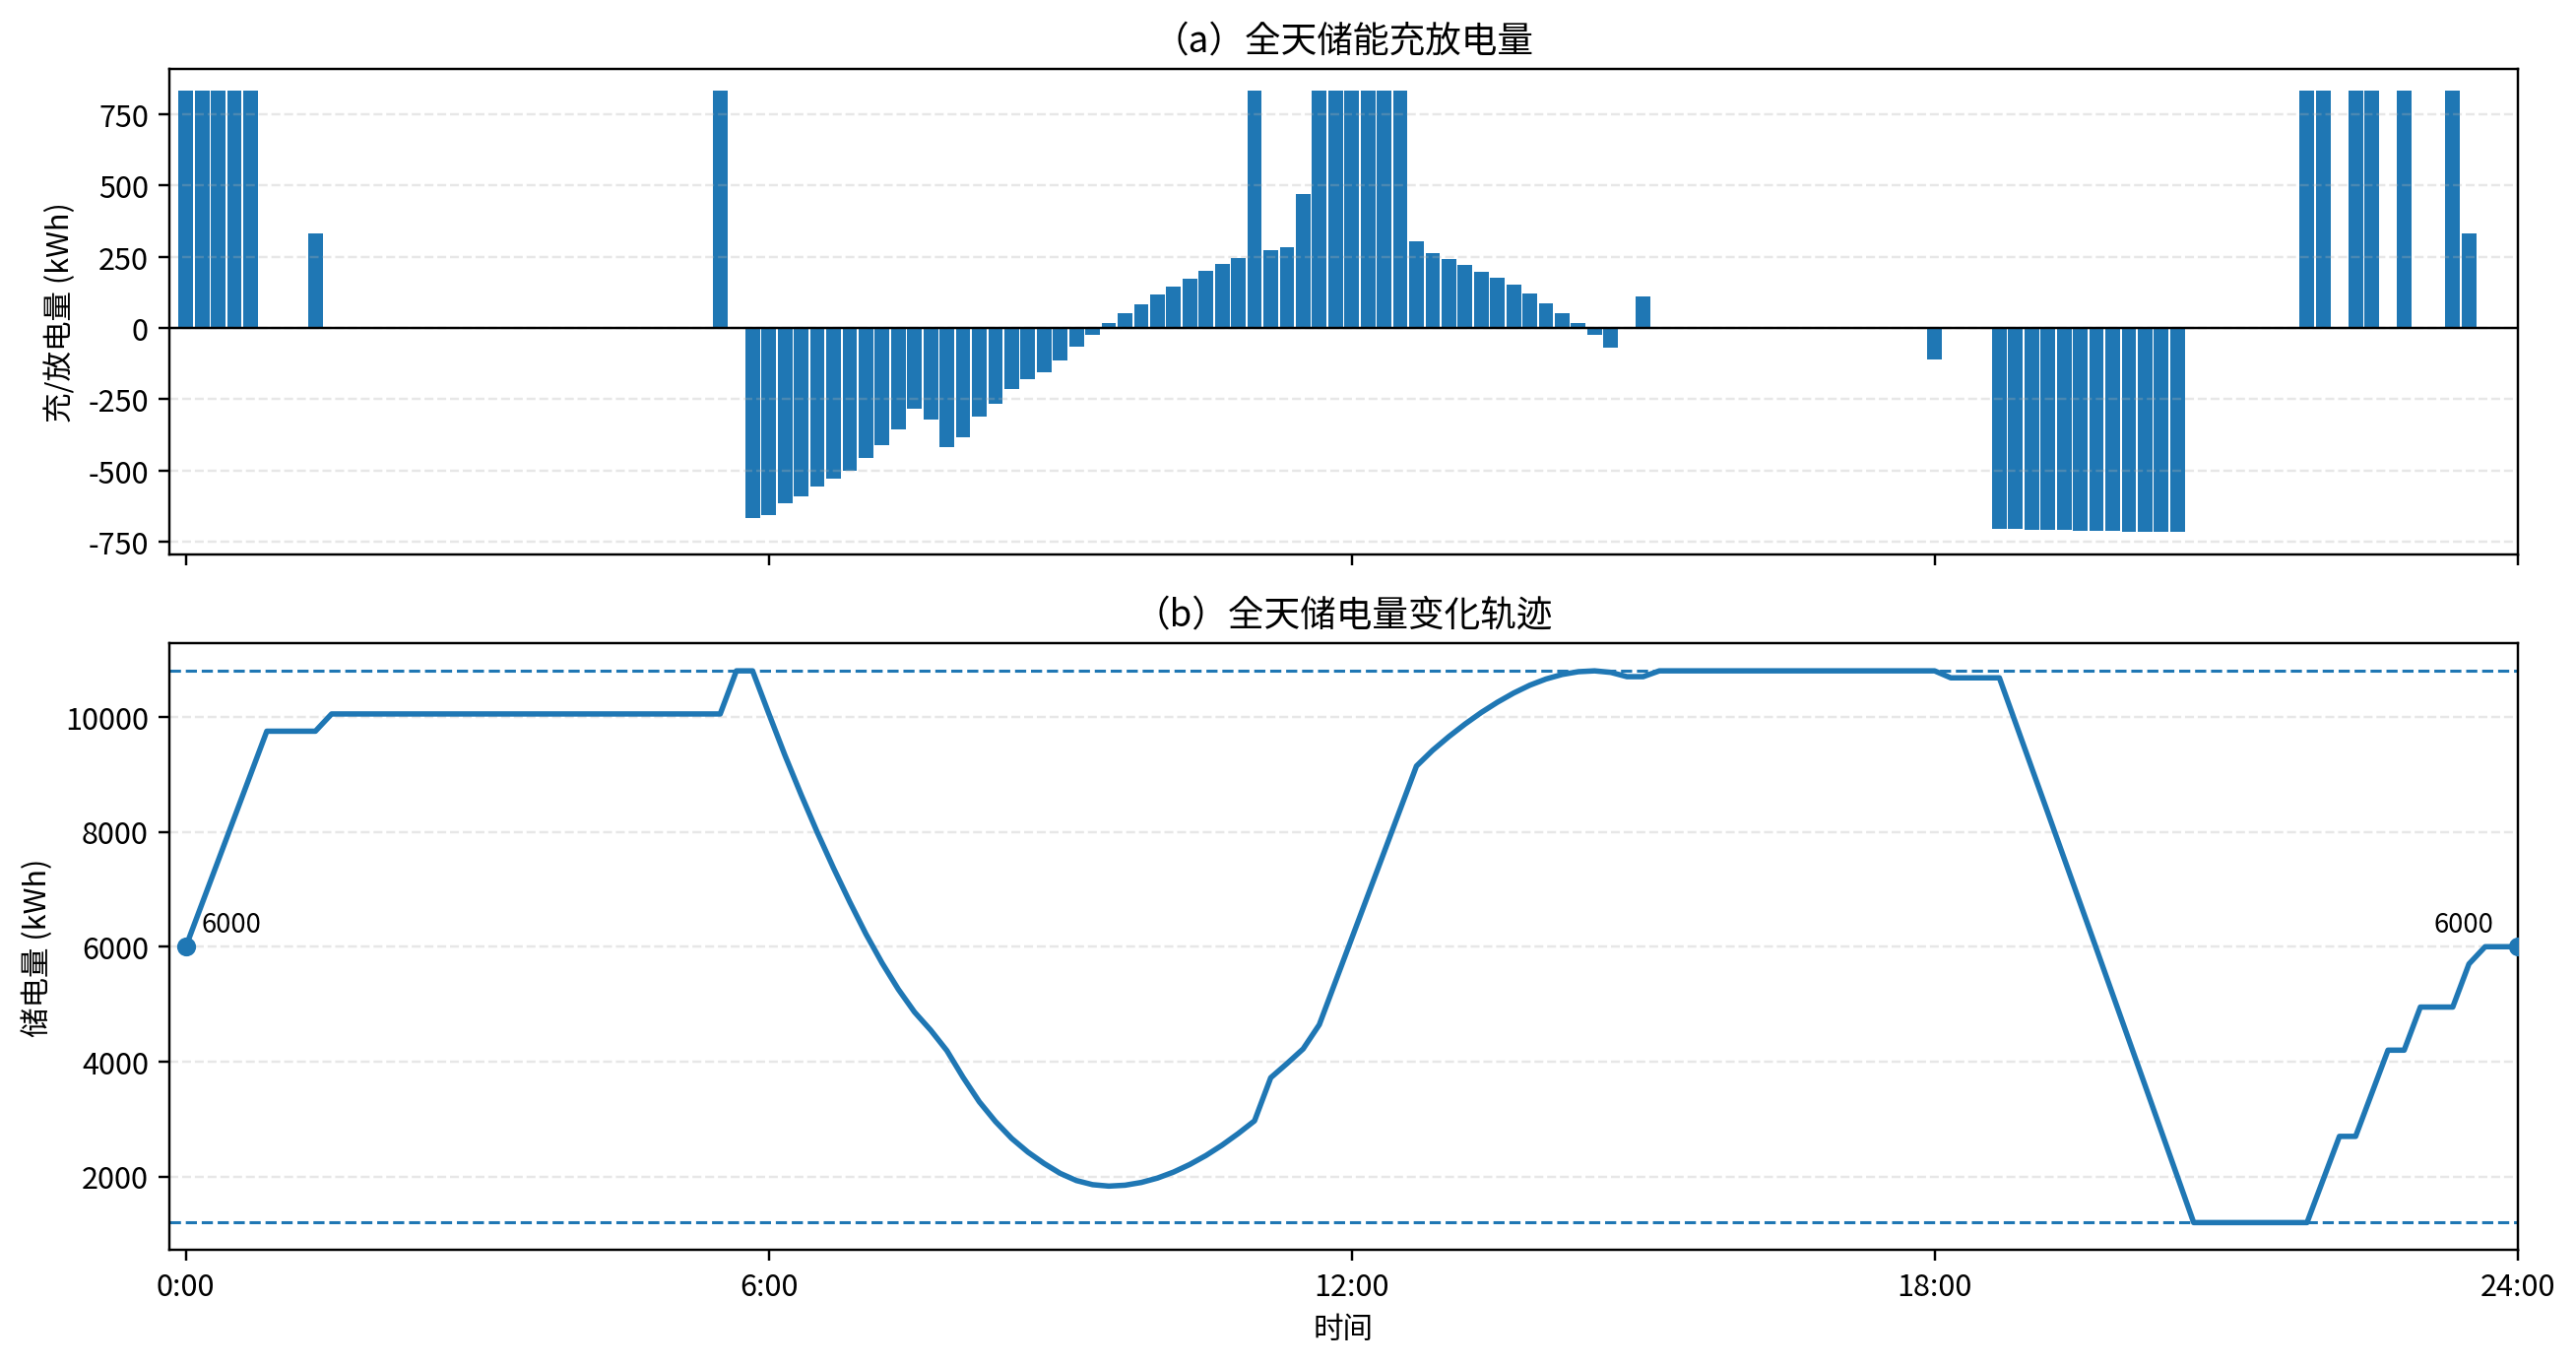
\includegraphics[width=0.95\textwidth]{figure/Q1.png}
    \caption{全天储能充放电及储电量变化轨迹}
    \label{fig:q1_dispatch}
\end{figure}
\subsection{模型检验与敏感性分析}

首先检验所得解的数值可行性。将最优解逐时回代能量平衡式和储电量递推式，
144 个时段的最大绝对残差分别为
$2.27\times10^{-13}\,\mathrm{kWh}$
和
$8.31\times10^{-13}\,\mathrm{kWh}$；
充、放电量上界、储电量边界及充放电互斥约束均满足，
且 $E_0=E_{144}=6000\,\mathrm{kWh}$。
对输出结果回读后重新计算购电费用，
与求解器目标值的误差仅为
$7.28\times10^{-12}$ 元，
验证了结果输出的一致性。
最优性方面，求解器返回 \texttt{OPTIMAL} 状态，
最终 MIP Gap 为 0，
因此所得方案在求解器设定的数值容差范围内达到所建 MILP 的全局最优。

进一步考察关键参数变化对最优购电费用 $J$ 的影响。
首先将充、放电单程效率同时取为 $0.85$、$0.90$ 和 $0.95$；
随后采用单因素扰动法，
在其余参数保持基准值不变的条件下，
分别将全天负荷和光伏出力整体调整 $\pm5\%$，
并保持各自日内曲线形状不变，即
\begin{equation}
    L_t^{\pm}=(1\pm0.05)L_t,\qquad
    S_t^{\pm}=(1\pm0.05)S_t.
    \label{eq:q1_sensitivity_perturbation}
\end{equation}

各扰动情形下的求解结果见表~\ref{tab:q1_sensitivity}。

\begin{table}[htbp]
    \centering
    \caption{关键参数敏感性分析结果}
    \label{tab:q1_sensitivity}
    \renewcommand{\arraystretch}{1.15}
    \begin{tabular}{cccc}
        \hline
        扰动因素 & 参数水平 & 最优购电费用/元 & 较基准变化 \\
        \hline
        单程效率 $\eta$ & $0.85$ & $36603.41$ & $+4.20\%$ \\
                        & $0.90$ & $35126.95$ & 基准 \\
                        & $0.95$ & $33767.03$ & $-3.87\%$ \\
        \hline
        负荷规模        & $-5\%$ & --- & $-10.18\%$ \\
                        & $+5\%$ & --- & $+10.55\%$ \\
        \hline
        光伏规模        & $-5\%$ & --- & $+4.47\%$ \\
                        & $+5\%$ & --- & $-4.26\%$ \\
        \hline
    \end{tabular}
\end{table}

由表~\ref{tab:q1_sensitivity} 可见，
在 $\eta\in[0.85,0.95]$ 的考察范围内，
单程效率提高对应的最优购电费用下降。
为进一步比较负荷与光伏整体规模变化对购电费用的相对影响，
定义中心差分相对敏感系数
\begin{equation}
    S_x=
    \frac{J_x^{+}-J_x^{-}}{0.1J_0},
    \qquad x\in\{L,\mathrm{PV}\},
    \label{eq:q1_relative_sensitivity}
\end{equation}
其中，$J_0$ 为基准最优费用，
$J_x^{+}$、$J_x^{-}$ 分别表示相应因素整体提高和降低 $5\%$ 时的最优费用。
计算得
\begin{equation}
    S_L=2.073,\qquad
    S_{\mathrm{PV}}=-0.873.
    \label{eq:q1_sensitivity_result}
\end{equation}

其中 $S_L>0$、$S_{\mathrm{PV}}<0$，
表明负荷规模增加将推高最优购电费用，
而光伏出力增加则降低外网购电需求及相应费用；又有
\begin{equation}
    |S_L|=2.073>|S_{\mathrm{PV}}|=0.873,
    \label{eq:q1_sensitivity_comparison}
\end{equation}
故在上述局部扰动范围内，
最优购电费用对负荷规模的相对敏感程度高于光伏出力。

\subsection{问题一小结}

针对日内电价、负荷及光伏预测功率均已知的日前调度情形，
本文在统一功率--电量口径的基础上，
建立了以全天购电费用最小为目标的源--荷--储协同调度 MILP 模型，
并通过能量平衡、储电量状态转移、充放电互斥及日周期边界等约束
保证调度方案的物理可行性。
求解结果表明，
全天计划购电量为 $59482.70\,\mathrm{kWh}$，
购电费用为 $35126.95$ 元，
全天无弃光，
且储能日末恢复至 $6000\,\mathrm{kWh}$ 的初始电量。
最优调度通过在低电价或光伏富余时段储能、
在高电价时段释放电量，
实现了光伏消纳与分时电价利用的跨时段协调。

数值检验表明，
所得方案满足全部模型约束，
并在求解器设定的数值容差范围内达到所建 MILP 的全局最优；
敏感性分析进一步表明，
在所考察的局部扰动范围内，
购电费用随单程储能效率提高而下降，
对负荷规模的相对敏感程度高于光伏出力。
由此，
所建模型能够在题设确定性条件下有效刻画微网源--荷--储之间的时序耦合关系，
并给出满足运行约束的日前经济调度方案。

\section{问题二的模型建立与求解}

\subsection{问题分析与数据处理}

问题二中，微网仍需于每日 $0{:}00$ 制定全天计划购电策略，但当日实际负荷与光伏功率在决策时尚未实现；若实际供能不足，缺口部分需按交易时刻正常电价的 $5$ 倍紧急购电。相较于问题一的确定性调度，本问进一步引入源荷不确定性，且净负荷低估导致的高价补购损失显著高于计划购电过量产生的成本。因此，每日 $0{:}00$ 需依据历史信息预测未来源荷，在不确定性场景下联合确定计划购电量与储能响应参数，日内再根据已实现的供需状态执行预先确定的储能反馈规则。故本文将问题二归结为\textbf{源荷不确定性下具有非对称补购损失的滚动随机调度问题}。

附件~2 分别以“日期$\times$日内时段”的形式给出全年小区负荷与光伏实际功率。记第 $d$ 日第 $t$ 时段的负荷功率和光伏功率分别为 $L_{d,t}$ 和 $P_{d,t}^{PV}$，二者均以 $\mathrm{kW}$ 计。将两张工作表按日期和时段展开，以 $(d,t)$ 为共同索引逐时配对，并将附件~1 的日内电价映射至相应时段；同时核查时间索引、缺失与重复记录以及源荷取值的物理合理性。时间尺度及功率--电量转换均沿用前文统一口径。

为保证历史回测与实际决策具有一致的信息边界，第 $d$ 日 $0{:}00$ 的预测、历史误差统计、场景构造及调度决策仅使用此前已经实现的信息，即$\mathcal I_d=\{L_{j,t},P_{j,t}^{PV}:j<d\}$
。第 $d$ 日及之后的真实源荷仅用于事后运行回放与结果评价。$1$ 月用于积累预测历史和样本外误差，自 $2$ 月 $1$ 日起进行正式滚动评价。


\subsection{负荷与光伏预测及联合随机场景构造}

\subsubsection{负荷与光伏功率预测}

随机调度既需要未来源荷的中心预测，也需要严格样本外预测误差以刻画不确定性。本文分别对负荷和光伏进行逐日滚动预测，以下用 $\widehat{\cdot}$ 表示预测值；多日前瞻中尚未实现的滞后特征均由前序预测递推生成，不使用未来真实观测。

负荷具有明显的日内及周周期特征，所以将周季节朴素模型
$\widehat L_{d,t}^{\mathrm{SNaive}}=L_{d-7,t}$
作为基准，并采用 LightGBM 刻画非线性变化。模型输入包括日内时段、星期与工作日属性，前 $1$、$2$、$7$ 日同刻负荷，以及过去 $7$ 日同刻负荷的均值和标准差。LightGBM 候选超参数依据 $1$ 月 $15$--$31$ 日首日前瞻的样本外负荷 MAE 确定，自 $2$ 月起固定；各日仅利用决策时已经获得的历史数据重新拟合。

光伏功率具有稳定的昼夜周期，但日际幅值波动较明显。以过去 $7$ 日同刻均值为基准，并利用最近 $28$ 日历史建立动态谐波回归--ARMA 模型。将 $10\,\mathrm{min}$ 序列连续编号为 $\ell$，有
$P_{\ell}^{PV}=\boldsymbol{\beta}^{\mathsf T}\mathbf h_{\ell}+\varepsilon_{\ell}$，
其中，$\mathbf h_{\ell}$ 为包含线性趋势、日周期谐波及其趋势交互项的特征向量，$\boldsymbol{\beta}$ 为回归系数，$\varepsilon_{\ell}$ 由低阶 ARMA 过程描述。谐波阶数在 $3$ 阶和 $6$ 阶中选择，AR、MA 阶数均在 $\{0,1\}$ 中搜索，并以 BIC 为主要准则、AIC 为辅助准则确定模型，同时对残差相关性和白噪声特征进行诊断。

为使预测评价体现紧急购电造成的非对称经济后果，以下记
$[x]_+=\max\{x,0\}$，并定义实际与预测净外部需求电量分别为
\[
Z_{d,t}
=
\left[
\Delta t\left(L_{d,t}-P_{d,t}^{PV}\right)
\right]_+,
\qquad
\widehat Z_{d,t}
=
\left[
\Delta t\left(\widehat L_{d,t}-\widehat P_{d,t}^{PV}\right)
\right]_+.
\]。
计划少购 $1\,\mathrm{kWh}$ 时，相较于正常提前购电将增加 $4p_t$ 的增量费用；计划多购 $1\,\mathrm{kWh}$ 且剩余电量无法回售时，损失为 $p_t$。据此定义辅助经济损失
\begin{equation}
    \mathcal L_{\mathrm{econ}}
    =
    \frac{1}{N_{\mathrm{eval}}}
    \sum_{d,t}
    \left[
        p_t\left(\widehat Z_{d,t}-Z_{d,t}\right)_+
        +
        4p_t\left(Z_{d,t}-\widehat Z_{d,t}\right)_+
    \right],
    \label{eq:q2_economic_loss}
\end{equation}
其中 $N_{\mathrm{eval}}$ 为参与评价的样本数。该指标仅用于衡量预测误差的非对称经济后果，不进入后续随机调度目标，也不等同于考虑储能跨时段耦合后的实际运行费用。

记负荷与光伏模型组成的联合预测方案为
$\boldsymbol{\kappa}_d=(\kappa_d^{L},\kappa_d^{PV})$。
各候选方案在相同的历史样本外区间上比较，以
$\mathcal L_{\mathrm{econ}}$ 为首要指标；对处于当前最优值 $1\%$ 相对容差内的候选，再依次比较净负荷、负荷和光伏的 MAE、RMSE。$1$ 月 $1$--$14$ 日用于积累初始历史，自 $1$ 月 $15$ 日起逐日生成并保存严格样本外预测及误差，为 $2$ 月起的随机场景构造提供历史依据。
\subsubsection{基于样本外误差的联合场景构造与尾部校准}

为保留负荷、光伏预测误差之间及连续时段间的相关性，
本文以同一历史预测起点下完整的源荷样本外误差轨迹作为场景构造单元。
记前瞻长度为 $K$ 日，$T=144K$。
历史起点 $j$ 的负荷、光伏误差分别为
\[
e_{j,h,t}^{L}
=
L_{j+h,t}-\widehat L_{j+h\mid j,t},
\qquad
e_{j,h,t}^{PV}
=
P_{j+h,t}^{PV}-\widehat P_{j+h\mid j,t}^{PV}.
\]
仅使用在第 $d$ 日决策前已完整实现的历史轨迹，
并优先选取近期样本构造经验场景池。

记场景 $s$ 对应历史起点为 $j_s$。
将其误差叠加至当前点预测，并令 $\tau=144h+t$，得到
\begin{equation}
\begin{array}{@{}lcl@{}}
L_{d+h,t}^{(s)}
&=&
\left[\widehat L_{d+h\mid d,t}+e_{j_s,h,t}^{L}\right]_+,
\\[3pt]
P_{d+h,t}^{PV,(s)}
&=&
\left[\widehat P_{d+h\mid d,t}^{PV}+e_{j_s,h,t}^{PV}\right]_+,
\\[3pt]
n_{\tau\mid d}^{(s)}
&=&
\Delta t
\left(
L_{d+h,t}^{(s)}-P_{d+h,t}^{PV,(s)}
\right).
\end{array}
\label{eq:q2_joint_scenario}
\end{equation}

为避免近期样本遗漏连续净负荷低估的高风险轨迹，
定义净负荷误差
$
e_{j,h,t}^{N}
=
\Delta t(e_{j,h,t}^{L}-e_{j,h,t}^{PV})
$
及累计供能压力
\begin{equation}
A_j
=
\max_{1\le m\le T}
\left[
\sum_{u=1}^{m}e_{j,u}^{N}
\right]_+ .
\label{eq:q2_tail_pressure}
\end{equation}
按 $A_j$ 排序，将最高的
$\rho_{\mathrm{tail}}=20\%$
历史轨迹划为尾部层，其余作为主体层。

当历史场景较多时，
分别对主体与尾部的标准化联合误差轨迹采用 $k$-medoids 缩减；
场景规模依据目标值、首日购电策略及尾部风险的稳定性确定，
必要时回退至完整经验场景池。
设尾部经验概率质量为
$
\omega_d=|\mathcal T_d|/|\mathcal J_d^{\mathrm{all}}|
$，
则两层内部按经验概率质量均匀赋权：
\begin{equation}
\pi_s
=
\begin{cases}
\dfrac{1-\omega_d}{S_d^{\mathrm{body}}},
& s\in\mathcal S_d^{\mathrm{body}},\\[6pt]
\dfrac{\omega_d}{S_d^{\mathrm{tail}}},
& s\in\mathcal S_d^{\mathrm{tail}},
\end{cases}
\qquad
\sum_{s=1}^{S_d}\pi_s=1 .
\label{eq:q2_scenario_probability}
\end{equation}

由此在控制场景规模的同时，
保留源荷误差的联合依赖、时间相关性及高供能压力尾部。
\subsection{不对称补购损失下的滚动随机调度模型}

\subsubsection{5 倍紧急购电机制下的报童模型分析}
\label{subsec:q2_newsvendor}

为揭示题设价格机制对应的非对称损失结构，暂忽略储能及跨时段耦合，考虑无储能单时段退化情形。记该时段计划购电量为 $g_t$，净外部需求电量为 $Z_t$。计划少购 $1\,\mathrm{kWh}$ 时，相较于正常提前购电产生的增量缺货损失为
\[
C_u=5p_t-p_t=4p_t;
\]
计划多购 $1\,\mathrm{kWh}$ 且剩余电量无法回售时，过量损失为
\[
C_o=p_t.
\]
记 $Q_{\alpha}(X)$ 为随机变量 $X$ 的 $\alpha$ 分位数，则经典报童模型的临界分位水平为
\begin{equation}
    \alpha^*
    =
    \frac{C_u}{C_u+C_o}
    =
    0.8,
    \qquad
    g_t^*
    =
    Q_{0.8}(Z_t).
    \label{eq:q2_newsvendor_quantile}
\end{equation}
因此，$0.8$ 分位由题设 $5$ 倍紧急购电价格直接确定。引入储能后，各时段通过储电量状态相互耦合，式~\eqref{eq:q2_newsvendor_quantile} 不再是逐时最优购电规则，但可作为完整随机调度中非对称补购风险的解析基准。


\subsubsection{滚动时域与日前策略}

若仅优化未来 $24\,\mathrm h$，
日末储电量的后续价值无法充分体现，
容易产生有限时域下的短视放电。
因此，本文比较 $48\,\mathrm h$ 与 $72\,\mathrm h$ 两种滚动前瞻窗口。
以 $72\,\mathrm h$ 结果为参照，
若二者首日计划购电量和期望费用的相对差异分别不超过
$2\%$ 和 $1\%$，
则采用计算量较低的 $48\,\mathrm h$ 窗口；
否则采用 $72\,\mathrm h$，
必要时回退至 $24\,\mathrm h$。
无论前瞻长度如何，每次仅实际执行首日 $144$ 个时段，
其余时段仅用于刻画日末储电量的继续价值。

第 $d$ 日 $0{:}00$ 在实际源荷实现前，
预先确定场景共享的日前策略
$x_d=\{g_{\tau\mid d},c_{\tau\mid d}^{p},
r_{\tau\mid d}^{p}\}_{\tau=1}^{T}$，
其中 $g_{\tau\mid d}$ 为计划外网购电量，
$c_{\tau\mid d}^{p}$、$r_{\tau\mid d}^{p}$
分别为充、放电响应上限，并满足
$g_{\tau\mid d}\ge0$、
$0\le c_{\tau\mid d}^{p},r_{\tau\mid d}^{p}\le Q_{\max}$。
上述策略参数在场景实现前确定并由所有场景共享，
实际充、放电方向及调用量则根据日内已经实现的供需状态确定，
从而保证决策的非前瞻性。


\subsubsection{基于历史误差的动态储电安全裕度}

连续出现净负荷低估时，储能可能在前部时段过早放电，从而削弱后续高需求阶段的补救能力。为此，本文在不改变储能物理下限的前提下，根据历史样本外预测误差设置时变安全裕度。

记 $\mathcal J_d^{R}$ 为截至第 $d$ 日 $0{:}00$ 已经完整形成首日前瞻误差、且与当前预测方案一致的历史预测起点集合。对
$j\in\mathcal J_d^{R}$，定义从第 $t$ 个时段起至当日结束可能经历的最大累计净负荷低估量
\begin{equation}
    H_{j,t}
    =
    \max_{t\le m\le144}
    \left[
        \sum_{u=t}^{m}
        e_{j,0,u}^{N}
    \right]_+,
    \qquad
    t=1,\ldots,144 .
    \label{eq:q2_future_pressure}
\end{equation}
据此设置第 $t$ 个时段的储电安全裕度
\begin{equation}
    R_{t\mid d}
    =
    \min
    \left\{
        E_{\max}-E_{\min},
        \frac{1}{\eta_d}
        Q_{0.8}
        \left(
            \{H_{j,t}:j\in\mathcal J_d^{R}\}
        \right)
    \right\}.
    \label{eq:q2_dynamic_reserve}
\end{equation}
其中，$1/\eta_d$ 用于将母线侧备用电量折算为电池侧储电量。这里采用的 $0.8$ 分位源于前述非对称补购损失，仅作为经济风险启发下的安全裕度参数，不解释为多时段储能问题的理论最优分位。

$R_{t\mid d}$ 在每日 $0{:}00$ 根据当时已实现历史一次确定，并仅作用于滚动窗口中实际执行的首日。为统一相对时段记号，令
\[
\widetilde R_{\tau\mid d}
=
\begin{cases}
R_{\tau\mid d}, & 1\le\tau\le144,\\
0, & 144<\tau\le T.
\end{cases}
\]


\subsubsection{负荷优先的非前瞻储能响应}

场景逐时实现后，定义计划购电后的即时净缺口
\[
\delta_{\tau\mid d}^{(s)}
=
n_{\tau\mid d}^{(s)}
-
g_{\tau\mid d}.
\]
记场景 $s$ 下实际充电量、实际放电量、紧急购电量和最终未利用电量分别为
$c_{\tau\mid d}^{(s)}$、
$r_{\tau\mid d}^{(s)}$、
$q_{\tau\mid d}^{(s)}$ 和
$w_{\tau\mid d}^{(s)}$。

当 $\delta_{\tau\mid d}^{(s)}>0$ 时，计划购电不足，优先在安全裕度允许范围内调用储能，其余缺口由紧急购电补足：
\begin{equation}
\left\{
\begin{aligned}
    c_{\tau\mid d}^{(s)}
    &=
    w_{\tau\mid d}^{(s)}
    =
    0,
    \\
    r_{\tau\mid d}^{(s)}
    &=
    \min
    \left\{
        r_{\tau\mid d}^{p},
        \delta_{\tau\mid d}^{(s)},
        \eta_d
        \left[
            E_{\tau-1\mid d}^{(s)}
            -
            E_{\min}
            -
            \widetilde R_{\tau\mid d}
        \right]_+
    \right\},
    \\
    q_{\tau\mid d}^{(s)}
    &=
    \delta_{\tau\mid d}^{(s)}
    -
    r_{\tau\mid d}^{(s)} .
\end{aligned}
\right.
\label{eq:q2_shortage_response}
\end{equation}

当 $\delta_{\tau\mid d}^{(s)}<0$ 时，满足负荷后仍存在剩余电量，优先在储能容量和预设响应上限允许范围内充电：
\begin{equation}
\left\{
\begin{aligned}
    r_{\tau\mid d}^{(s)}
    &=
    q_{\tau\mid d}^{(s)}
    =
    0,
    \\
    c_{\tau\mid d}^{(s)}
    &=
    \min
    \left\{
        c_{\tau\mid d}^{p},
        -\delta_{\tau\mid d}^{(s)},
        \frac{
            E_{\max}-E_{\tau-1\mid d}^{(s)}
        }{\eta_c}
    \right\},
    \\
    w_{\tau\mid d}^{(s)}
    &=
    -\delta_{\tau\mid d}^{(s)}
    -
    c_{\tau\mid d}^{(s)} .
\end{aligned}
\right.
\label{eq:q2_surplus_response}
\end{equation}
当 $\delta_{\tau\mid d}^{(s)}=0$ 时，上述四类响应量均为 $0$。因此，紧急购电仅用于弥补当期实际供能缺口，不用于储能充电。

上述反馈仅依赖当前已经实现的净负荷及上一时段储电状态，不调用未来真实源荷，因而满足非前瞻性。受附件数据 $10\,\mathrm{min}$ 时间分辨率限制，本文以区间聚合电量刻画该响应过程，不假定在区间起点已获知整个区间的最终净负荷。


\subsubsection{场景运行约束与随机优化目标}

对于任一场景 $s$ 和时段 $\tau$，母线侧能量平衡、储能状态转移及储电量边界分别满足
\begin{equation}
\begin{aligned}
    g_{\tau\mid d}
    +
    r_{\tau\mid d}^{(s)}
    +
    q_{\tau\mid d}^{(s)}
    &=
    n_{\tau\mid d}^{(s)}
    +
    c_{\tau\mid d}^{(s)}
    +
    w_{\tau\mid d}^{(s)},
    \\
    E_{\tau\mid d}^{(s)}
    &=
    E_{\tau-1\mid d}^{(s)}
    +
    \eta_c c_{\tau\mid d}^{(s)}
    -
    \frac{r_{\tau\mid d}^{(s)}}{\eta_d},
    \\
    E_{\min}
    &\le
    E_{\tau\mid d}^{(s)}
    \le
    E_{\max}.
\end{aligned}
\label{eq:q2_physical_constraints}
\end{equation}
其中，
$w_{\tau\mid d}^{(s)}$
表示不存在回售收益的最终未利用电量，既可能来自富余光伏，也可能来自最终未被利用的计划购电，因此不简单解释为弃光量。储能参数沿用问题一，即
$E_{\min}=1200\,\mathrm{kWh}$、
$E_{\max}=10800\,\mathrm{kWh}$、
$\eta_c=\eta_d=0.9$。

本文将 $1$ 月作为预测历史和误差库的预热区间，期间储能不主动调度，且不计入正式评价费用。因此，结合题设初始储电量，正式评价开始时取
\[
E_{\mathrm{Feb\,1},0}
=
6000\,\mathrm{kWh}.
\]
自 $2$ 月 $1$ 日起，各场景均从当日实际日初储电量出发，
\[
E_{0\mid d}^{(s)}
=
E_{d,0},
\]
并将上一日实际运行末态连续传递至下一日日初。

在上述联合随机场景及非前瞻反馈机制下，第 $d$ 日滚动窗口以计划购电费用和期望紧急购电费用之和最小为目标：
\begin{equation}
    \boxed{
    \min_{x_d}J_d
    =
    \sum_{\tau=1}^{T}
        p_{\tau}g_{\tau\mid d}
    +
    \sum_{s=1}^{S_d}
        \pi_s
        \sum_{\tau=1}^{T}
            5p_{\tau}q_{\tau\mid d}^{(s)}
    }.
    \label{eq:q2_stochastic_objective}
\end{equation}
其中，计划购电始终按正常电价计费，未利用部分不产生退款或回售收益；紧急购电按对应时段正常电价的 $5$ 倍计费。上述分段响应关系可通过辅助变量和指示约束进行等价线性化，从而得到有限场景下的混合整数线性规划模型。由于日内反馈映射的形式预先给定，所得解为上述参数化非前瞻策略类中的最优方案。

为与滚动决策机制保持一致，每日求解后仅实施窗口首日 $144$ 个时段的
$g_{d,t}$、$c_{d,t}^{p}$、$r_{d,t}^{p}$ 及当日 $0{:}00$ 已确定的安全裕度 $R_{d,t}$，并将当日实际负荷和光伏逐时输入同一反馈规则。记由此产生的实际紧急购电量为
$q_{d,t}^{\mathrm{real}}$，则第 $d$ 日实际购电费用按
\begin{equation}
    C_d^{\mathrm{real}}
    =
    \sum_{t=1}^{144}
    \left(
        p_tg_{d,t}
        +
        5p_tq_{d,t}^{\mathrm{real}}
    \right)
    \label{eq:q2_real_cost}
\end{equation}
核算。当日 $24{:}00$ 的实际储电量作为下一日日初状态。上述过程仅规定滚动执行与费用统计口径，具体运行轨迹及经济性结果在后文统一分析。
```

\subsection{调度结果与经济性分析}

对2025年2月1日至12月31日进行逐日滚动求解，并以当日实际负荷与光伏功率进行回放。
四个指定日期的计划购电、储能运行及紧急购电结果分别见
表~\ref{tab:q2_purchase}--\ref{tab:q2_emergency}。

% ======================== 表1 ========================
\begin{table}[H]
    \centering
    \caption{指定日期计划购电结果}
    \label{tab:q2_purchase}
    \scriptsize
    \setlength{\tabcolsep}{2.6pt}
    \renewcommand{\arraystretch}{0.88}
    \begin{tabular}{c*{6}{r}rr}
        \toprule
        日期
        & 10:00--10:10 & 12:00--12:10 & 14:00--14:10
        & 16:00--16:10 & 18:00--18:10 & 20:00--20:10
        & 全天购电量 & 购电费 \\
        \midrule
        3.20  & 30.77  & 647.12 & 0.00 & 491.08 & 678.98 & 47.68
              & 65354.44  & 41469.88 \\
        6.21  & 0.00   & 0.00   & 0.00 & 266.24 & 489.62 & 13.81
              & 45357.23  & 27013.07 \\
        9.23  & 0.00   & 0.00   & 0.00 & 550.68 & 751.57 & 57.08
              & 68930.26  & 44583.94 \\
        12.21 & 174.61 & 975.14 & 6.81 & 882.64 & 745.52 & 8.16
              & 102661.44 & 67637.24 \\
        \bottomrule
    \end{tabular}

    {\scriptsize 注：购电量单位为 kWh，购电费单位为元。}
\end{table}

\vspace{-1mm}

% ======================== 表2 ========================
\begin{table}[H]
    \centering
    \caption{指定日期储能运行结果}
    \label{tab:q2_storage}
    \scriptsize
    \setlength{\tabcolsep}{2.8pt}
    \renewcommand{\arraystretch}{0.88}
    \begin{tabular}{c*{8}{r}}
        \toprule
        \multirow{2}{*}{时段}
        & \multicolumn{2}{c}{3.20}
        & \multicolumn{2}{c}{6.21}
        & \multicolumn{2}{c}{9.23}
        & \multicolumn{2}{c}{12.21} \\
        \cmidrule(lr){2-3}
        \cmidrule(lr){4-5}
        \cmidrule(lr){6-7}
        \cmidrule(lr){8-9}
        & 充电 & 放电 & 充电 & 放电 & 充电 & 放电 & 充电 & 放电 \\
        \midrule
        0:00--4:00
        & 1704.88 & 78.66
        & 1757.12 & 0.00
        & 1897.73 & 0.00
        & 2393.00 & 0.00 \\

        4:00--8:00
        & 1113.39 & 4525.67
        & 822.94 & 2877.36
        & 1713.90 & 3205.68
        & 939.07 & 1265.42 \\

        8:00--12:00
        & 6041.43 & 2338.27
        & 4777.70 & 0.00
        & 2703.45 & 1896.62
        & 5958.49 & 4546.23 \\

        12:00--16:00
        & 2460.12 & 386.54
        & 0.00 & 0.00
        & 3031.42 & 403.62
        & 2989.26 & 2196.68 \\

        16:00--20:00
        & 257.99 & 5216.80
        & 0.00 & 4683.45
        & 47.84 & 5616.23
        & 0.00 & 5232.62 \\

        20:00--24:00
        & 3259.65 & 2866.88
        & 8487.28 & 2445.85
        & 7866.80 & 2869.97
        & 7791.67 & 2742.77 \\
        \midrule
        $E_{0:00}$
        & \multicolumn{2}{c}{8609.12}
        & \multicolumn{2}{c}{7375.09}
        & \multicolumn{2}{c}{8505.83}
        & \multicolumn{2}{c}{8646.30} \\

        $E_{24:00}$
        & \multicolumn{2}{c}{4837.48}
        & \multicolumn{2}{c}{10517.11}
        & \multicolumn{2}{c}{8494.07}
        & \multicolumn{2}{c}{8950.96} \\
        \bottomrule
    \end{tabular}

    {\scriptsize 注：充、放电量及储电量单位均为 kWh。}
\end{table}

\vspace{-1mm}

% ======================== 表3 ========================
\begin{table}[H]
    \centering
    \caption{微网在指定日期的紧急购电量}
    \label{tab:q2_emergency}
    \scriptsize
    \setlength{\tabcolsep}{3.1pt}
    \renewcommand{\arraystretch}{0.88}
    \begin{tabular}{crcrcrcr}
        \toprule
        \multicolumn{2}{c}{2025.3.20}
        & \multicolumn{2}{c}{2025.6.21}
        & \multicolumn{2}{c}{2025.9.23}
        & \multicolumn{2}{c}{2025.12.21} \\
        \cmidrule(lr){1-2}
        \cmidrule(lr){3-4}
        \cmidrule(lr){5-6}
        \cmidrule(lr){7-8}
        时间段 & 购电量
        & 时间段 & 购电量
        & 时间段 & 购电量
        & 时间段 & 购电量 \\
        \midrule
        15:50--16:10 & 28.13
        & -- & 0
        & 17:30--17:40 & 12.00
        & -- & 0 \\

        21:20--21:30 & 12.13
        & -- & --
        & 19:20--19:30 & 0.98
        & -- & -- \\

        23:30--23:40 & 13.31
        & -- & --
        & 20:20--20:30 & 0.88
        & -- & -- \\

        -- & --
        & -- & --
        & 20:50--21:00 & 26.76
        & -- & -- \\
        \bottomrule
    \end{tabular}

    {\scriptsize 注：紧急购电量单位为 kWh，“--”表示无对应紧急购电时段。}
\end{table}

% ======================== 结果图 ========================
\begin{figure}[htbp]
    \centering
    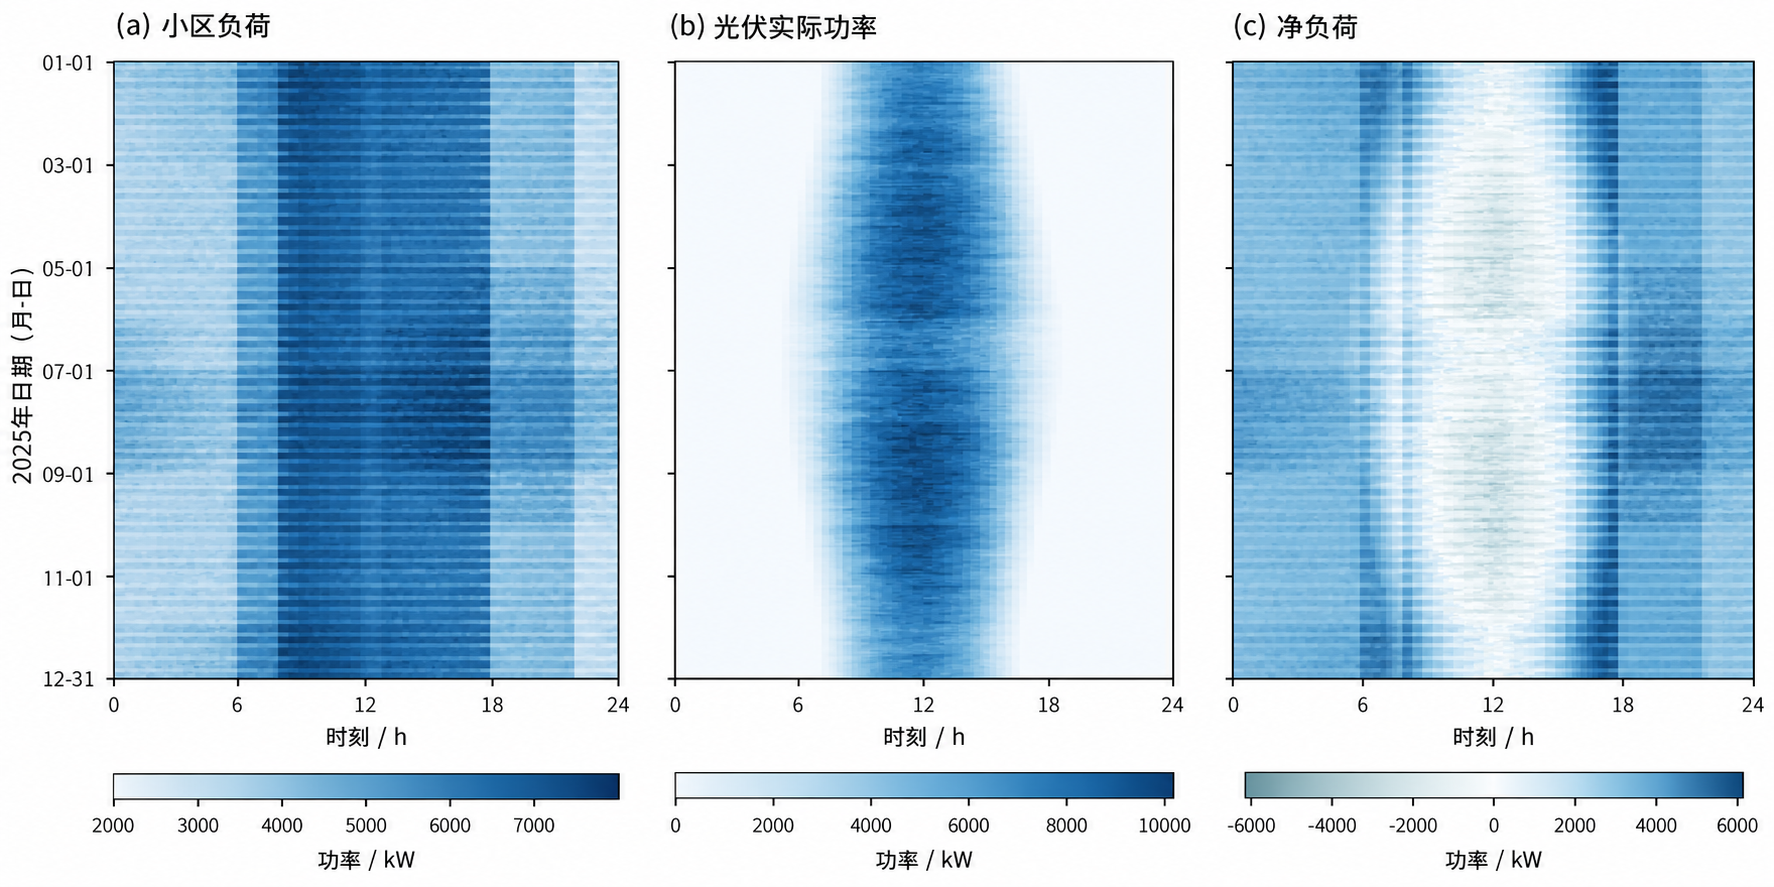
\includegraphics[width=0.94\textwidth]{figure/Q2.png}
    \caption{2025年小区负荷、光伏实际功率与净负荷日内分布}
    \label{fig:q2_source_load}
\end{figure}

图~\ref{fig:q2_source_load}表明，
全年负荷具有较稳定的日内周期，光伏出力集中于白昼并随季节变化；
二者共同作用下，净负荷在午间明显降低，而早晚时段整体较高，
且相同时刻仍存在显著日际波动。
这一特征说明源荷过程同时具有可预测的周期结构与不可忽略的随机扰动，
与本文采用滚动预测和随机场景刻画不确定性的建模思路一致。

评价期内计划购电量累计为
$2.1654\times10^7\,\mathrm{kWh}$，
紧急购电量为
$1.3026\times10^5\,\mathrm{kWh}$，
仅占实际外购电量的$0.60\%$；
但紧急购电费用为$67.72$万元，
占总购电费用$1419.63$万元的$4.77\%$。
四个指定日期中，仅3月20日和9月23日出现少量紧急购电。
结果表明，所建策略能够将供能缺口控制在较小范围；
同时，紧急购电量占比较低而费用占比明显较高，
说明5倍补购机制下净负荷低估具有显著的非对称经济代价。
\subsection{参数敏感性分析}

选取常规日、高预测误差日、高紧急购电日和高系统压力日进行单因素敏感性实验。
为考察动态储电安全裕度的影响，在基准安全裕度 $R_{t|d}$ 上引入无量纲倍率
$\beta_R$，令
\[
    R_{t|d}^{(\beta)}
    =
    \beta_R R_{t|d},
\]
其中基准情形取 $\beta_R=1$。
同时改变尾部场景比例 $\rho_{\mathrm{tail}}$，
分别考察安全裕度强度与尾部场景配置对实际运行结果的影响，结果见表~\ref{tab:q2_sensitivity}。

\begin{table}[H]
    \centering
    \caption{问题二参数敏感性分析结果}
    \label{tab:q2_sensitivity}
    \scriptsize
    \setlength{\tabcolsep}{4.0pt}
    \renewcommand{\arraystretch}{0.92}
    \begin{tabular}{ccccc}
        \toprule
        参数 & 取值
        & 成本变化/\%
        & 紧急购电量/kWh
        & 最低储电量/kWh \\
        \midrule

        \multirow{3}{*}{$\beta_R$}
        & 0.8
        & $0.399\,[-1.406,\,6.262]$
        & $4460.32\,[20.29,\,13899.00]$
        & $1521.92\,[1288.96,\,1972.20]$ \\

        & 1.0
        & $0$
        & $4345.46\,[13.97,\,12344.95]$
        & $1545.00\,[1311.20,\,1968.73]$ \\

        & 1.2
        & $-0.123\,[-1.053,\,0.257]$
        & $4274.12\,[20.29,\,12436.10]$
        & $1588.95\,[1333.44,\,2032.61]$ \\

        \midrule

        \multirow{3}{*}{$\rho_{\mathrm{tail}}$}
        & 10\%
        & $-0.737\,[-2.745,\,7.567]$
        & $4397.11\,[11.96,\,14167.85]$
        & $1403.48\,[1311.20,\,1784.57]$ \\

        & 20\%
        & $0$
        & $4345.46\,[13.97,\,12344.95]$
        & $1545.00\,[1311.20,\,1968.73]$ \\

        & 30\%
        & $2.134\,[-1.296,\,8.387]$
        & $4428.57\,[10.65,\,12868.47]$
        & $1483.55\,[1311.20,\,1728.25]$ \\

        \bottomrule
    \end{tabular}

    {\scriptsize 注：表中为4个代表日的
    “中位数[最小值，最大值]”，成本变化均相对于同日基准方案。}
\end{table}

由表~\ref{tab:q2_sensitivity}可见，
$\beta_R$提高至$1.2$时成本变化中位数仅为$-0.123\%$，
表明模型对安全裕度参数总体较稳定；
降低$\beta_R$则在部分高风险工况下明显增加补购代价。

相比之下，$\rho_{\mathrm{tail}}$更为敏感：
提高至$30\%$后成本变化中位数增至$2.134\%$，最大增幅达$8.387\%$。
因此，基准设置$\beta_R=1.0$、$\rho_{\mathrm{tail}}=20\%$
在代表工况下能够较好兼顾经济性与风险控制。



\section{问题三的模型建立与求解}
\subsection{问题分析与数据预处理}

问题三在问题二基础上增加 $0{:}00$、$6{:}00$、$12{:}00$ 和 $18{:}00$ 四个预报与决策节点。新预报到达后，已执行决策保持不变，并以当前实际储电量为新的初始状态重新优化未来策略。由于增购、减购及紧急购电对应不同结算代价，只有当预报更新带来的预期运行成本下降超过调整代价时，策略调整才产生净收益。考虑储能的跨时段耦合，本文建立\textbf{基于负荷--光伏联合预测误差场景的四时点随机滚动经济调度模型}。

负荷预测沿用问题二每日 $0{:}00$ 生成的因果预测，日内仅更新附件~3 的光伏预报。四个节点均采用前向 $24\,\mathrm{h}$ 优化窗口，仅下一滚动决策时点前的决策实际执行，之后部分作为前瞻信息评估后续运行成本。整点光伏预报按发布时间和预测提前量映射至目标时刻后插值至 $10\,\mathrm{min}$ 尺度。历史场景由\textbf{相同决策节点下、同一历史日期且对应相同目标时段的负荷与光伏预测误差轨迹配对构成}，并仅选取整段目标区间均已实现的历史轨迹。1 月按相同滚动调度与结算机制连续推进储电量；尚无可用历史误差轨迹时采用确定性滚动，随历史样本积累逐步启用随机场景模型，自 2 月 1 日起进行正式评价。
\subsection{基于联合历史误差的随机场景构造}

负荷与光伏预测误差共同决定净负荷的不确定性。若对二者及各时段分别独立抽样，
将破坏源荷误差之间及各时段之间的依赖结构。因此，本文以
\textbf{同一历史日期中与当前节点对应的前向 $24\,\mathrm{h}$ 源荷联合误差轨迹}
作为场景构造单元。

设当前为第 $d$ 日节点
\[
k\in\{0,6,12,18\},
\]
记 $h=1,\ldots,H$ 为自节点 $k$ 起的相对 $10\,\mathrm{min}$ 目标步，
其中 $H=144$。候选历史起点 $j<d$ 须同时满足负荷样本外预测可得，
且对应前向 $24\,\mathrm{h}$ 真实轨迹在当前节点前已完整实现。

固定第 $d$ 日选定的负荷预测器，采用该预测器在历史日期 $j$ 上仅利用当时可用信息
得到的样本外预测；光伏误差则由与当前节点相同发布时间下的历史预报计算。定义
\begin{equation}
e_{j,k,h}^{L}
=
L_{j,k,h}^{\mathrm{real}}
-
\widehat{L}_{j,k,h}^{\,0},
\qquad
e_{j,k,h}^{PV}
=
P_{j,k,h}^{PV,\mathrm{real}}
-
\widehat{P}_{j,k,h|k}^{PV}.
\label{eq:q3_joint_error}
\end{equation}
其中，对负荷误差而言，$k$ 仅用于确定前向 $24\,\mathrm{h}$ 误差轨迹的截取起点，
其预测发布时间仍固定为当日 $0{:}00$。两类误差按同一历史日期及相同相对目标时段对齐，
其中负荷误差来自该日 $0{:}00$ 的预测，光伏误差来自节点 $k$ 发布的预报；
当 $k>0$ 时，相应轨迹可自然跨越至次日。

将历史联合误差叠加至当前预测，得到场景 $s$ 下
\begin{equation}
L_{h,s}^{(d,k)}
=
\max\left\{
0,\,
\widehat{L}_{d,k,h}^{\,0}
+
e_{j,k,h}^{L}
\right\},
\label{eq:q3_scenario_load}
\end{equation}

\begin{equation}
P_{h,s}^{PV,(d,k)}
=
\max\left\{
0,\,
\widehat{P}_{d,k,h|k}^{PV}
+
e_{j,k,h}^{PV}
\right\},
\label{eq:q3_scenario_pv}
\end{equation}

\begin{equation}
n_{h,s}^{(d,k)}
=
\Delta t
\left(
L_{h,s}^{(d,k)}
-
P_{h,s}^{PV,(d,k)}
\right).
\label{eq:q3_scenario_netload}
\end{equation}

为兼顾历史样本的时效性与场景数量，候选池依次采用最近 $28$、$56$、$84$ 日
及全部可用历史，并选取首个满足场景规模要求的时间窗口。进一步按前向
$24\,\mathrm{h}$ 预测光伏总电量
\begin{equation}
Z_{j,k}
=
\Delta t
\sum_{h=1}^{H}
\widehat{P}_{j,k,h|k}^{PV}
\label{eq:q3_pv_energy_indicator}
\end{equation}
的三分位数划分低、中、高三个区间，从当前 $Z_{d,k}$ 所在区间开始筛选；
若样本不足，则依次并入相邻区间。记条件化后的候选轨迹数为 $M_{d,k}$。

若 $M_{d,k}>S^\star$，在固定发布时间 $k$ 下，分别对各相对目标步上的净负荷误差
进行标准化，并以标准化轨迹间的欧氏距离进行场景缩减。定义净负荷误差
\begin{equation}
e_{j,k,h}^{N}
=
e_{j,k,h}^{L}
-
e_{j,k,h}^{PV},
\label{eq:q3_netload_error}
\end{equation}
并考虑较大的正向净负荷预测误差更易造成供电缺口，引入仅用于尾部筛选的
价格加权代理评分
\begin{equation}
R_{j,k}
=
\sum_{h=1}^{H}
p_{d,k,h}
\left[e_{j,k,h}^{N}\right]_+
\Delta t,
\label{eq:q3_tail_score}
\end{equation}
其中，$p_{d,k,h}$ 为当前节点后第 $h$ 个目标时段的电价。
$R_{j,k}$ 不等同于实际紧急购电费用；由于紧急购电价格中的系数 $5$
对所有轨迹的排序均相同，故在该评分中省略。

正式场景数取
\[
S^\star=20.
\]
当 $M_{d,k}>S^\star$ 时，首先保留 $R_{j,k}$ 最大的两条尾部轨迹，
再对其余样本采用 $k$-medoids 进行缩减；当 $M_{d,k}\le S^\star$ 时，
则保留全部候选轨迹。

将所有候选轨迹归入距离最近的代表轨迹。若代表场景 $s$ 覆盖 $m_s$ 条候选轨迹，
则赋予概率
\begin{equation}
\pi_s
=
\frac{m_s}{M_{d,k}},
\qquad
\sum_s \pi_s = 1.
\label{eq:q3_scenario_probability}
\end{equation}

场景缩减仅用于选择代表历史轨迹并确定其概率，最终输入随机优化模型的仍为
相应历史日期的\textbf{原始配对源荷误差轨迹}。由此，在控制计算规模的同时，
能够保留源荷误差的联合依赖、时序相关结构及高缺口尾部信息。

\subsection{四时点随机经济滚动优化模型}

\subsubsection{滚动时域与承诺执行机制}

问题三在 $0{:}00$、$6{:}00$、$12{:}00$、$18{:}00$ 四个节点获得新的光伏预报。
本文沿用当日 $0{:}00$ 基于当时可用信息生成的 $48\,\mathrm h$ 负荷预测，
日内不再更新，以覆盖最晚至次日 $18{:}00$ 的滚动时域；
各节点结合最新光伏预报、当前实际储电量及第~5.2~节构造的随机场景，
对未来 $24\,\mathrm h$ 重新优化。

沿用相对步长 $h=1,\ldots,H$，其中 $H=144$。
对 $k\in\{6,12,18\}$，记当前节点至当日 $24{:}00$ 的剩余时段数为
$H_k^{\mathrm{day}}=6(24-k)$，并划分
\begin{equation}
\mathcal B=\{1,\ldots,36\},
\qquad
\mathcal P_k=\{37,\ldots,H_k^{\mathrm{day}}\},
\qquad
\mathcal C_k=\{H_k^{\mathrm{day}}+1,\ldots,H\}.
\label{eq:q3_horizon_partition}
\end{equation}

其中，$\mathcal B$ 为下一预报到达前的承诺执行区间，
$\mathcal P_k$ 为当日后续前瞻区间，
$\mathcal C_k$ 为跨日继续区间；
当 $k=18$ 时，$\mathcal P_k=\varnothing$。
仅 $\mathcal B$ 内的决策在当前节点锁定，其余部分仅用于后续经济价值评估。

对于题目未明确的多次调整结算方式，
本文采用最终生效购电量相对当日 $0{:}00$ 原计划进行一次结算的解释，
后续滚动优化与实际费用核算均统一采用该口径。


\subsubsection{参数化因果储能策略与物理约束}

记 $g_{d,t}^{0}$ 为第 $d$ 日 $0{:}00$ 制定的原计划，
并以
\[
g_{d,k,h}^{0}
=
g_{d,\,6k+h}^{0}
\]
表示节点 $k$ 后第 $h$ 个当日目标时段对应的原计划量，
其中 $h\le H_k^{\mathrm{day}}$。

设 $g_{d,k,h}^{(k)}$ 为承诺区间的调整后绝对购电量，
$\widetilde g_{d,k,h}^{(k)}$ 为后续前瞻代理量，统一记
\begin{equation}
\gamma_h^{(d,k)}
=
\begin{cases}
g_{d,k,h}^{(k)},
& h\in\mathcal B,\\[1mm]
\widetilde g_{d,k,h}^{(k)},
& h\in\mathcal P_k\cup\mathcal C_k.
\end{cases}
\label{eq:q3_gamma}
\end{equation}

其中 $k=0$ 时取
$\gamma_h^{(d,0)}=g_{d,h}^{0}$，且
\[
0
\le
\gamma_h^{(d,k)}
\le
\Delta t\max_s L_{h,s}^{(d,k)}
+
Q_{\max}.
\]

为避免不同场景利用尚未实现的未来信息，
$\gamma_h^{(d,k)}$、$\bar c_h^{(d,k)}$ 和 $\bar r_h^{(d,k)}$
均由节点 $k$ 预先确定并由各场景共享，其中
\[
0
\le
\bar c_h^{(d,k)},\,
\bar r_h^{(d,k)}
\le
Q_{\max}.
\]

令场景净缺口
\[
x_{h,s}^{(d,k)}
=
n_{h,s}^{(d,k)}
-
\gamma_h^{(d,k)},
\]
则储能响应为
\begin{equation}
\begin{aligned}
r_{h,s}^{(d,k)}
&=
\min\left\{
\bar r_h^{(d,k)},
\left[x_{h,s}^{(d,k)}\right]_+,
\eta_d
\left(
E_{h-1,s}^{(d,k)}
-
E_{\min}
\right)
\right\},
\\
c_{h,s}^{(d,k)}
&=
\min\left\{
\bar c_h^{(d,k)},
\left[-x_{h,s}^{(d,k)}\right]_+,
\frac{
E_{\max}
-
E_{h-1,s}^{(d,k)}
}{
\eta_c
}
\right\}.
\end{aligned}
\label{eq:q3_storage_response}
\end{equation}

进一步令
\[
y_{h,s}^{(d,k)}
=
n_{h,s}^{(d,k)}
+
c_{h,s}^{(d,k)}
-
\gamma_h^{(d,k)}
-
r_{h,s}^{(d,k)},
\]
则紧急购电量和未利用剩余电量分别为
\[
q_{h,s}^{\mathrm{em},(d,k)}
=
\left[y_{h,s}^{(d,k)}\right]_+,
\qquad
u_{h,s}^{(d,k)}
=
\left[-y_{h,s}^{(d,k)}\right]_+,
\]
从而自动满足能量平衡。

这里 $u$ 可能同时包含光伏富余和计划购电偏高产生的剩余电量，
故不将其简单解释为弃光量。

储电量满足
\begin{equation}
\begin{gathered}
E_{h,s}^{(d,k)}
=
E_{h-1,s}^{(d,k)}
+
\eta_c c_{h,s}^{(d,k)}
-
\frac{
r_{h,s}^{(d,k)}
}{
\eta_d
},
\\
E_{\min}
\le
E_{h,s}^{(d,k)}
\le
E_{\max},
\qquad
E_{0,s}^{(d,k)}
=
E_{d,k}^{\mathrm{real}}.
\end{gathered}
\label{eq:q3_storage_state}
\end{equation}

上述反馈关系表示区间内实时因果控制在 $10\,\mathrm{min}$ 尺度上的聚合近似。


\subsubsection{四时点随机经济优化目标}

记 $p_{d,k,h}$ 为节点 $k$ 向前第 $h$ 个目标时段对应的电价。
在 $0{:}00$ 节点尚不存在购电调整，采用风险中性目标
\begin{equation}
\min J_{d,0}
=
\sum_{h=1}^{H} p_{d,0,h}g_{d,h}^{0}
+
\sum_s \pi_s
\left(
\sum_{h=1}^{H} 5p_{d,0,h}q_{h,s}^{\mathrm{em},(d,0)}
-
\lambda_{E,0}^{(d)}E_{H,s}^{(d,0)}
\right).
\label{eq:q3_objective_0}
\end{equation}

其中，$\lambda_{E,k}^{(d)}$ 为窗口末端单位储电量的继续价值，
由当前日期以前最近至多 $28$ 个已完整实现的同节点历史窗口
进行储能边际价值有限差分估计并取中位数，
以减弱有限时域导致的末端过度放电。

$g^0$ 为 $0{:}00$ 滚动随机优化得到的基准计划；
由于未显式构造后三次预报更新对应的完整多阶段场景树，
因此不将其解释为完整四阶段随机规划的一阶段最优策略。

对 $k\in\{6,12,18\}$，
承诺区间内相对原计划的增量调整费用定义为
\begin{equation}
A_h^{\mathrm{adj},(d,k)}
=
p_{d,k,h}
\left[
1.5
\left(
g_{d,k,h}^{(k)}
-
g_{d,k,h}^{0}
\right)_+
-
0.5
\left(
g_{d,k,h}^{0}
-
g_{d,k,h}^{(k)}
\right)_+
\right].
\label{eq:q3_adjustment_cost}
\end{equation}

当日后续区间令
$\widetilde A_h^{\mathrm{sur},(d,k)}$
表示将上式中的 $g_{d,k,h}^{(k)}$
替换为 $\widetilde g_{d,k,h}^{(k)}$
后得到的同形式代理费用；
跨日区间按正常购电费用估计。
于是节点 $k$ 的滚动目标为
\begin{equation}
\begin{aligned}
\min J_{d,k}
={}&
\sum_{h\in\mathcal B}
A_h^{\mathrm{adj},(d,k)}
+
\sum_{h\in\mathcal P_k}
\widetilde A_h^{\mathrm{sur},(d,k)}
+
\sum_{h\in\mathcal C_k}
p_{d,k,h}
\widetilde g_{d,k,h}^{(k)}
\\
&+
\sum_s\pi_s
\left[
\sum_{h=1}^{H}
5p_{d,k,h}
q_{h,s}^{\mathrm{em},(d,k)}
-
\lambda_{E,k}^{(d)}
E_{H,s}^{(d,k)}
\right].
\end{aligned}
\label{eq:q3_objective_k}
\end{equation}

其中，$\mathcal B$ 中的费用对应当前实际调整，
$\mathcal P_k$ 与 $\mathcal C_k$ 中的变量仅用于评估后续经济影响，
不直接计入当前真实结算。


\subsubsection{实际执行与费用核算}

令
\[
\mathcal T_0=\{1,\ldots,36\},\qquad
\mathcal T_6=\{37,\ldots,72\},
\]
\[
\mathcal T_{12}=\{73,\ldots,108\},\qquad
\mathcal T_{18}=\{109,\ldots,144\},
\]
并约定
\[
g_{d,t}^{(0)}
=
g_{d,t}^{0}.
\]

则当天最终生效购电量统一表示为
\begin{equation}
g_{d,t}^{\mathrm{eff}}
=
g_{d,t}^{(k)},
\qquad
t\in\mathcal T_k,
\quad
k\in\{0,6,12,18\}.
\label{eq:q3_effective_purchase}
\end{equation}

实际运行按附件~2 的真实轨迹及对应承诺区间冻结的储能反馈参数
逐 $10\,\mathrm{min}$ 回放，
记所得真实紧急购电量为
$q_{d,t}^{\mathrm{em,real}}$；
日末实际储电量直接传递为次日初始状态。

在本文采用的单次结算口径下，
第 $d$ 日实际总费用可统一写为
\begin{equation}
C_d^{\mathrm{total}}
=
\sum_{t=1}^{144}
p_t
\left[
g_{d,t}^{0}
+
1.5
\left(
g_{d,t}^{\mathrm{eff}}
-
g_{d,t}^{0}
\right)_+
-
0.5
\left(
g_{d,t}^{0}
-
g_{d,t}^{\mathrm{eff}}
\right)_+
+
5q_{d,t}^{\mathrm{em,real}}
\right].
\label{eq:q3_actual_total_cost}
\end{equation}

前瞻代理费用与终端价值仅参与滚动决策，不计入实际费用。
上述分段线性关系可通过辅助变量与 $0$--$1$ 指示变量转化为有限场景下的
确定性等价 MILP，并采用整数规划求解器求解。
求解所得策略进一步通过真实轨迹逐时回放，对能量平衡、储能状态及运行边界进行复核。

\subsection{调度结果与多时点预报价值分析}

对 2025 年 2--12 月共 334 个评价日进行逐日滚动回放。
按照题目要求，选取 2025.3.20、2025.6.21、2025.9.23 和
2025.12.21 四个指定日期，其购电、储能运行及紧急购电结果分别见
表~\ref{tab:q3_specified_purchase}--表~\ref{tab:q3_emergency}，
完整购电策略保存于 \texttt{result3.xlsx}。

%========================================================
% 表1：指定日期购电结果
%========================================================
\begin{table}[H]
    \centering
    \caption{指定日期的购电量及全天购电结果}
    \label{tab:q3_specified_purchase}
    \scriptsize
    \setlength{\tabcolsep}{3.1pt}
    \renewcommand{\arraystretch}{1.12}
    \resizebox{\textwidth}{!}{
    \begin{tabular}{c*{8}{c}}
        \toprule
        日期
        & 10:00--10:10
        & 12:00--12:10
        & 14:00--14:10
        & 16:00--16:10
        & 18:00--18:10
        & 20:00--20:10
        & 全天购电量
        & 全天购电费 \\
        & \multicolumn{6}{c}{最终有效购电量/$\mathrm{kWh}$}
        & /$\mathrm{kWh}$
        & /元 \\
        \midrule

        2025.3.20
        & 0.00
        & 566.62
        & 0.00
        & 522.26
        & 698.98
        & 0.00
        & 65903.58
        & 42648.52 \\

        2025.6.21
        & 0.00
        & 0.00
        & 0.00
        & 186.37
        & 425.50
        & 0.00
        & 35641.56
        & 21866.93 \\

        2025.9.23
        & 0.00
        & 0.00
        & 0.00
        & 553.88
        & 650.13
        & 64.19
        & 66878.06
        & 44795.01 \\

        2025.12.21
        & 0.00
        & 1003.27
        & 0.00
        & 883.43
        & 687.10
        & 0.00
        & 94774.99
        & 62048.55 \\
        \bottomrule
    \end{tabular}}
\end{table}

%========================================================
% 表2：指定日期储能结果
%========================================================
\begin{table}[H]
    \centering
    \caption{指定日期储能设备的充放电量及日初、日末储电量}
    \label{tab:q3_specified_storage}
    \scriptsize
    \setlength{\tabcolsep}{3.0pt}
    \renewcommand{\arraystretch}{1.12}
    \resizebox{\textwidth}{!}{
    \begin{tabular}{ccccccccc}
        \toprule
        日期
        & 0:00--4:00
        & 4:00--8:00
        & 8:00--12:00
        & 12:00--16:00
        & 16:00--20:00
        & 20:00--24:00
        & $E_{0:00}$
        & $E_{24:00}$ \\
        & \multicolumn{6}{c}{充电量/放电量（$\mathrm{kWh}$）}
        & \multicolumn{2}{c}{储电量（$\mathrm{kWh}$）} \\
        \midrule

        2025.3.20
        & $133.35/508.92$
        & $901.75/5890.14$
        & $4378.90/2655.22$
        & $5787.54/314.20$
        & $258.97/5219.82$
        & $9711.84/2939.04$
        & 10328.72
        & 9909.02 \\

        2025.6.21
        & $203.99/3015.96$
        & $395.14/4836.61$
        & $9782.58/0.00$
        & $0.00/0.00$
        & $0.00/4223.79$
        & $8233.35/2485.90$
        & 10181.53
        & 10754.81 \\

        2025.9.23
        & $4640.26/0.00$
        & $971.29/5277.50$
        & $5123.57/1896.62$
        & $4037.29/410.90$
        & $66.66/6072.21$
        & $5426.35/2624.57$
        & 5910.21
        & 6058.21 \\

        2025.12.21
        & $431.33/389.22$
        & $1939.55/1813.82$
        & $5061.21/6733.62$
        & $7291.73/2397.78$
        & $35.81/5611.76$
        & $9713.67/2908.49$
        & 10142.37
        & 10107.58 \\
        \bottomrule
    \end{tabular}}
\end{table}

%========================================================
% 表3：指定日期紧急购电
%========================================================
\begin{table}[H]
    \centering
    \caption{指定日期的紧急购电量}
    \label{tab:q3_emergency}
    \scriptsize
    \setlength{\tabcolsep}{5.0pt}
    \renewcommand{\arraystretch}{1.10}

    \begin{tabular}{cccccccc}
        \toprule
        \multicolumn{2}{c}{2025.3.20}
        & \multicolumn{2}{c}{2025.6.21}
        & \multicolumn{2}{c}{2025.9.23}
        & \multicolumn{2}{c}{2025.12.21} \\
        \cmidrule(lr){1-2}
        \cmidrule(lr){3-4}
        \cmidrule(lr){5-6}
        \cmidrule(lr){7-8}

        时间段 & 购电量
        & 时间段 & 购电量
        & 时间段 & 购电量
        & 时间段 & 购电量 \\
        & /kWh
        & & /kWh
        & & /kWh
        & & /kWh \\
        \midrule

        09:30--10:00 & 122.16
        & -- & --
        & 20:50--21:10 & 40.85
        & 12:50--13:00 & 9.60 \\

        20:00--20:10 & 12.61
        & -- & --
        & 21:20--21:40 & 36.87
        & 19:50--20:00 & 16.43 \\

        21:20--21:30 & 7.76
        & -- & --
        & -- & --
        & -- & -- \\

        21:40--21:50 & 18.23
        & -- & --
        & -- & --
        & -- & -- \\
        \bottomrule
    \end{tabular}
\end{table}
由表~\ref{tab:q3_specified_purchase}--表~\ref{tab:q3_emergency} 可见，
滚动策略能够依据新预报持续修正购电量，并通过储能充放电吸收源荷偏差；
多数偏差可由购电调整与储能共同消化，仅在调节余量不足时产生紧急购电，
其中 2025.6.21 全天未发生紧急购电。
为进一步展示预报更新对实际决策的作用过程，
选取题目指定日期 2025.3.20 的完整运行轨迹，如图~\ref{fig:q3_dispatch} 所示。

%========================================================
% 真实数据绘制的代表日调度图
%========================================================
\begin{figure}[H]
    \centering
    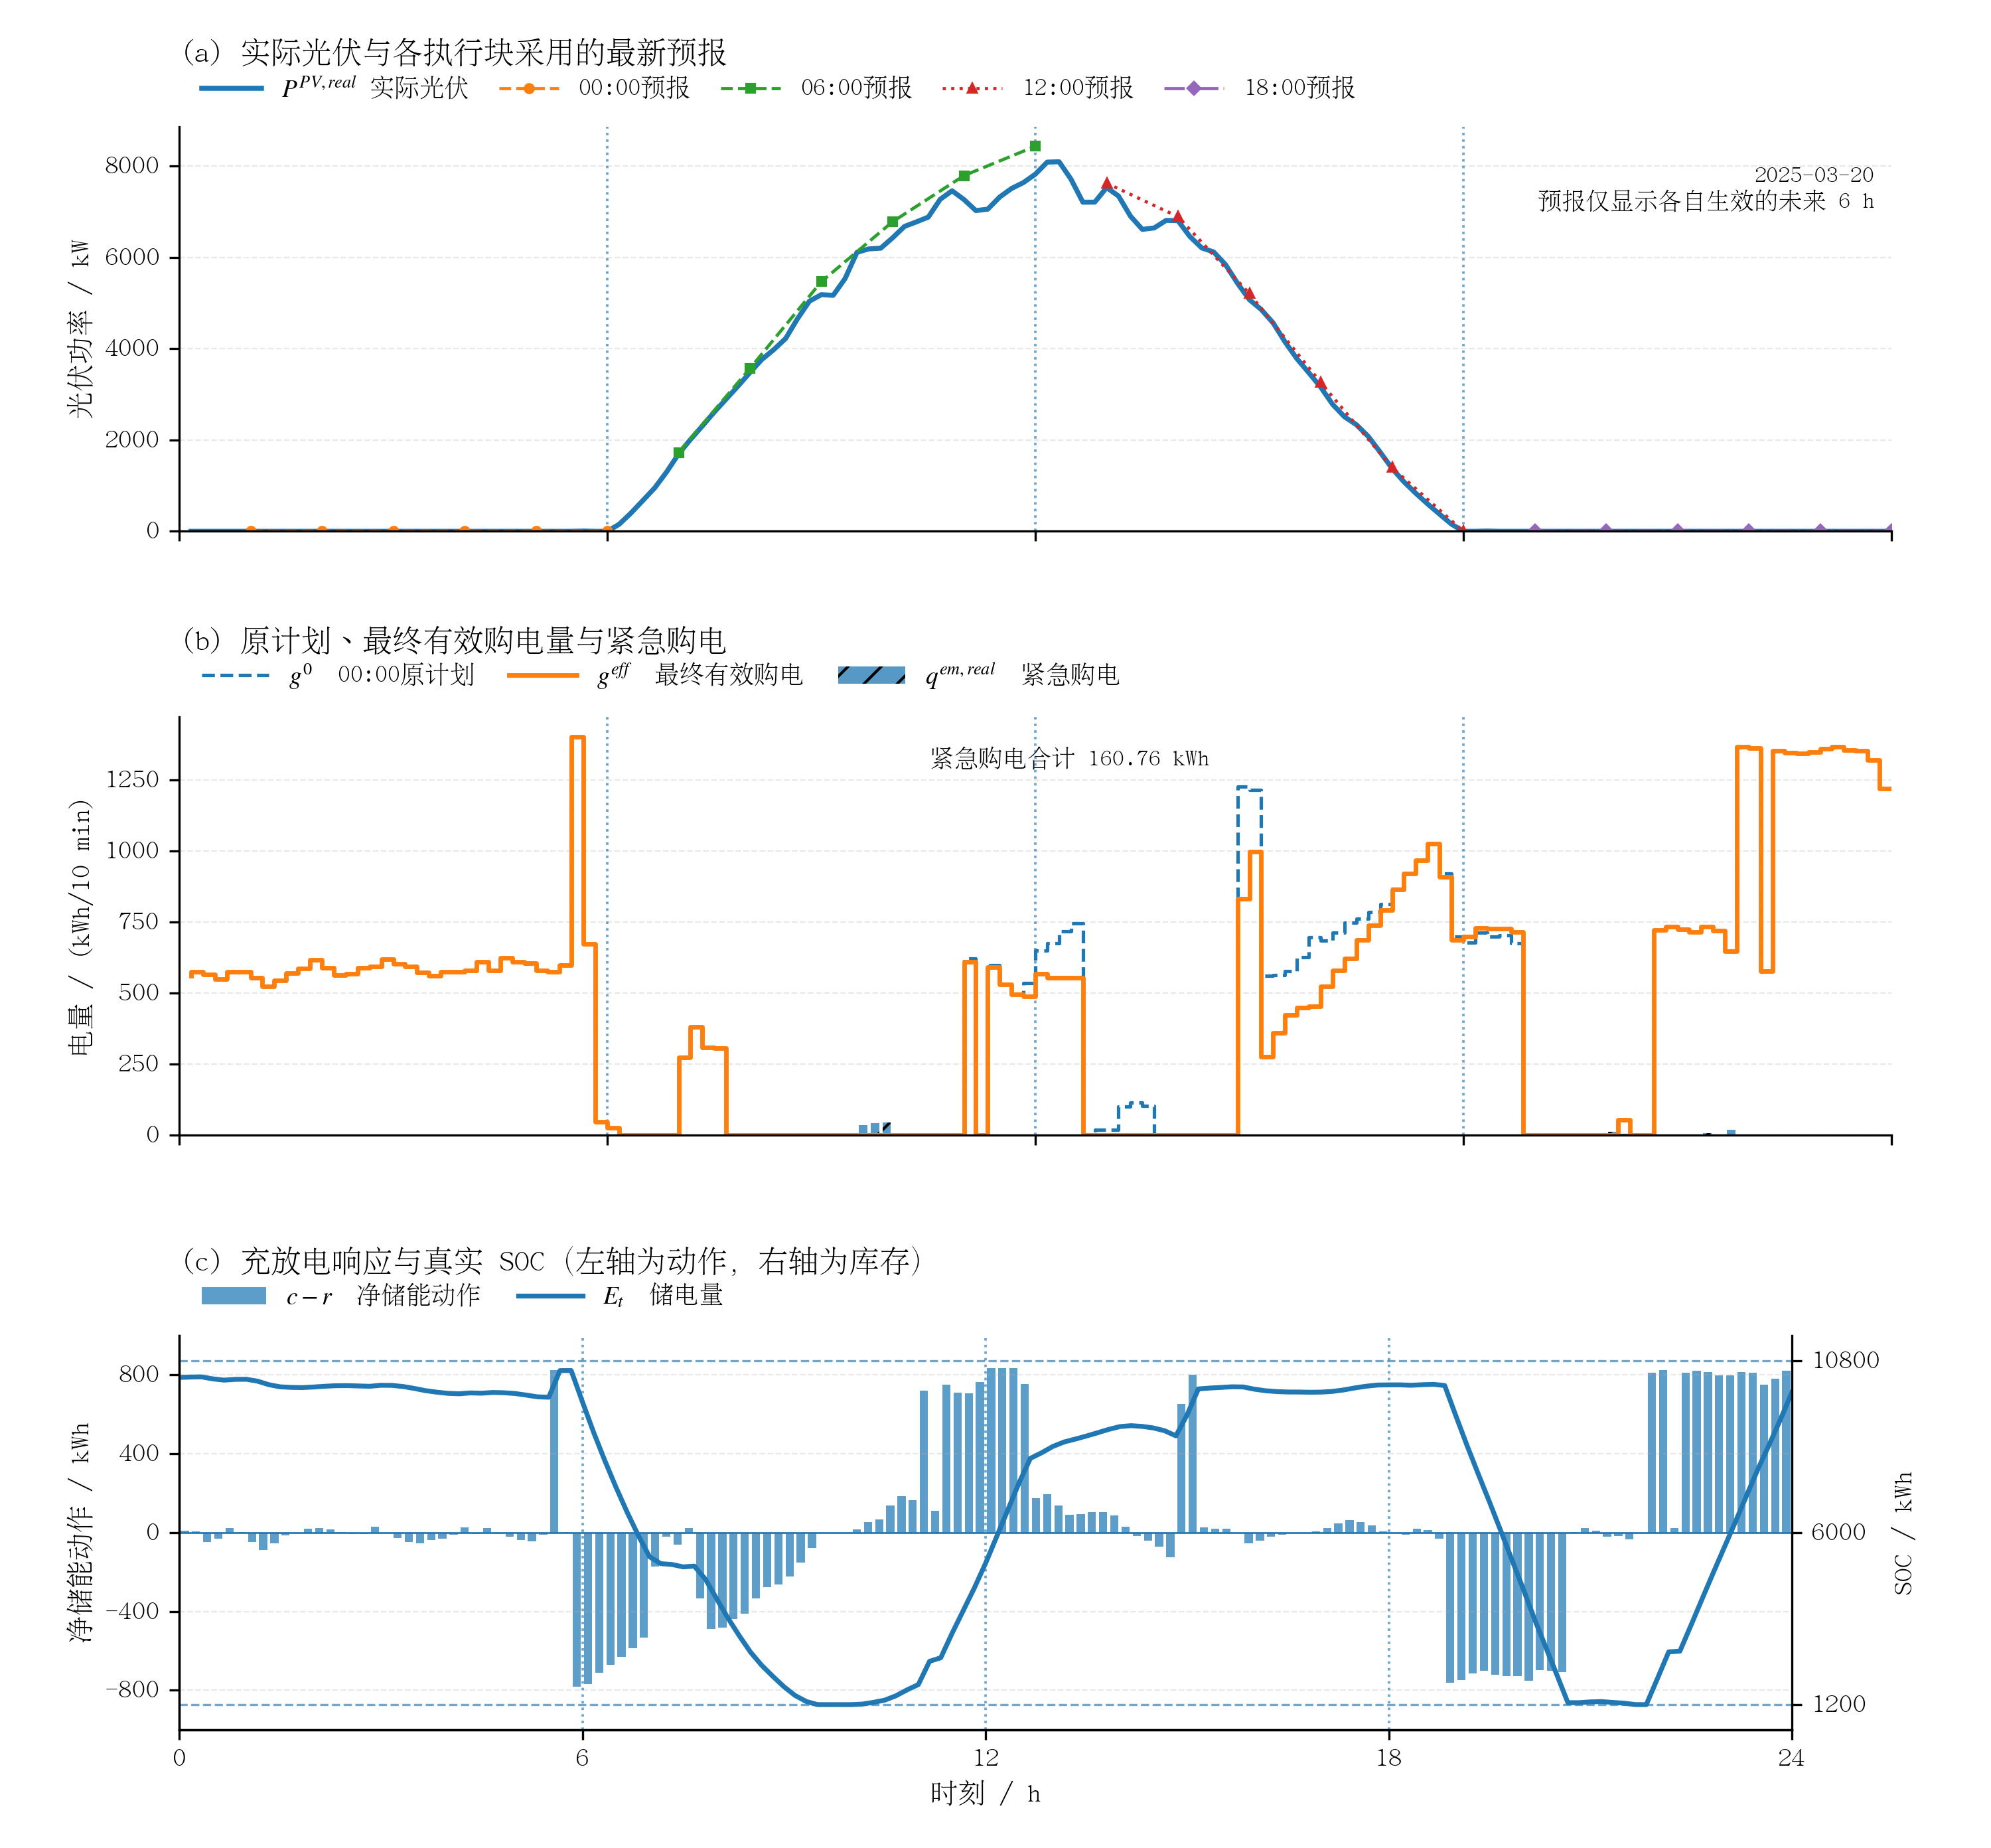
\includegraphics[width=0.96\textwidth]{figure/q3_dispatch_typical.png}
    \caption{2025.3.20 多时点预报更新下的购电与储能调度轨迹}
    \label{fig:q3_dispatch}
\end{figure}

图~\ref{fig:q3_dispatch} 表明，新预报到达后，后续购电计划随之修正，
储能通过充放电协同吸收源荷偏差；代表日仅发生
$160.76\,\mathrm{kWh}$ 紧急购电，且全过程满足储能运行约束。

在相邻预报共同覆盖的 $18\,\mathrm h$ 区间内，
$6{:}00$、$12{:}00$ 和 $18{:}00$ 更新后的光伏预测 MAE
分别下降 $47.94\%$、$67.95\%$ 和 $31.50\%$，
其中 $12{:}00$ 的信息增益最明显。
全年回放中，四时点滚动策略使实际总费用由
$1419.63$ 万元降至 $1338.77$ 万元，降低 $5.70\%$；
紧急购电量由 $13.03$ 万 $\mathrm{kWh}$ 降至
$5.26$ 万 $\mathrm{kWh}$，降低 $59.62\%$，
且 334 个评价日中有 269 日费用更低。
因此，日内预报更新具有实际应用价值，其中 $6{:}00$ 和 $12{:}00$
作用较为显著；$18{:}00$ 的当日直接作用较弱，
但考虑储能跨时段耦合仍予以保留。
上述成本改善为预报更新、状态反馈与滚动优化共同作用的综合收益。


\subsection{模型检验与敏感性分析}

将调度结果逐时回代后，能量平衡、储能容量及充放电功率约束均满足。
进一步选取代表工况，对场景数、尾部场景保留数及终端价值进行单因素扰动。
对于第~5.3.3~节由历史数据估计得到的基准终端价值
$\lambda_{E,k}^{(d)}$，引入无量纲倍率 $\beta_E$，令
\[
    \lambda_{E,k}^{(d,\beta)}
    =
    \beta_E \lambda_{E,k}^{(d)},
\]
其中基准情形取 $\beta_E=1$。
各参数扰动结果见表~\ref{tab:q3_sensitivity}。

\begin{table}[H]
    \centering
    \caption{问题三关键参数局部敏感性分析}
    \label{tab:q3_sensitivity}
    \scriptsize
    \setlength{\tabcolsep}{4.2pt}
    \renewcommand{\arraystretch}{1.10}

    \begin{tabular}{lcccc}
        \toprule
        参数设置
        & $\Delta C$ 中位数/\%
        & $\Delta C$ 范围/\%
        & $\Delta Q_{\rm em}$ 中位数/kWh
        & $E_{24}$ 中位数/kWh \\
        \midrule

        基准：$S=20,\ S_{\rm tail}=2,\ \beta_E=1.0$
        & $0.00$
        & $[0.00,\ 0.00]$
        & $0.00$
        & $8194.72$ \\

        $S=10$
        & $+2.50$
        & $[-1.44,\ +6.16]$
        & $+435.91$
        & $8782.59$ \\

        $S=28$
        & $-2.31$
        & $[-5.32,\ -0.12]$
        & $-130.65$
        & $5335.32$ \\

        $S_{\rm tail}=0$
        & $+0.30$
        & $[-0.77,\ +1.02]$
        & $+1.43$
        & $8191.06$ \\

        $S_{\rm tail}=4$
        & $+0.29$
        & $[+0.08,\ +0.67]$
        & $+100.05$
        & $8271.17$ \\

        $\beta_E=0.8$
        & $-6.05$
        & $[-9.28,\ -1.91]$
        & $+2.99$
        & $1236.51$ \\

        $\beta_E=1.2$
        & $+0.33$
        & $[-0.43,\ +0.90]$
        & $-85.77$
        & $8835.78$ \\

        \bottomrule
    \end{tabular}

    \vspace{1mm}
    \footnotesize
    \parbox{0.96\textwidth}{
    注：结果基于常规、高预测更新、高调整成本和高风险四类代表日；
    $\Delta C$、$\Delta Q_{\rm em}$ 分别表示相对基准方案的实际总费用
    和紧急购电量变化。
    }
\end{table}

由表~\ref{tab:q3_sensitivity} 可见，
尾部场景保留数变化对实际费用影响较小，
而场景规模变化会引起一定费用波动。
当 $\beta_E=0.8$ 时，窗口末端储电量明显下降，
说明终端价值项能够有效抑制有限滚动时域下的短视放电。
总体而言，模型在所考察代表工况下具有较好的局部稳定性。









\section{问题四的模型建立与求解}
\subsection{问题分析与数据处理}
问题四在问题二、问题三的基础上进一步考虑外网电价的实时波动。
问题~4-2 与问题~4-3 分别沿用前文的源荷预测、储能运行及购电调整机制，
并进一步引入未来电价的不确定性。
由于计划购电、调整购电和紧急购电均按对应交易时刻电价结算，
电价波动不仅改变各时段的购电成本，
也会改变源荷预测偏差所对应的经济损失，
并影响储能跨时段转移电量的价值。

尤其当净负荷偏高与电价偏高同时出现时，
供能不足将对应更高的紧急补购成本；
若将价格与净负荷分别独立处理，
可能低估此类联合不利状态的运行风险。
因此，本文在前述调度框架上进一步刻画价格与净负荷的联合不确定性，
并据此分别建立波动电价下的日前分布鲁棒调度模型
与四时点分布鲁棒滚动调度模型。

附件~4 以“日期$\times$日内时段”的宽表形式给出全年实时电价。
本文按日期和时段展开价格序列，
以 $(d,t)$ 为索引与附件~2 的源荷实际轨迹、
前文生成的净负荷预测以及附件~3 的四时点光伏预报逐时对齐。
核查结果表明，附件~4 共包含 $365$ 日、每日 $144$ 个时段的完整记录，
未发现缺失或重复数据。
按照前述非前瞻原则，
每一决策节点仅保留此前已经实现的电价作为历史样本，
节点之后的真实电价在实现前不进入预测、场景构造及优化模型。

为确定后续不确定性描述方式，进一步考察价格的时序结构及其与净负荷的联合变化。
电价的 $1$ 日、$7$ 日和 $14$ 日同刻相关系数分别为
$0.9335$、$0.9820$ 和 $0.9745$，
显示出较强的周周期结构。
采用 $7$ 日同刻差分削弱共同周期成分后，
价格与净负荷异常量的相关系数仍为 $0.6695$；
当净负荷异常进入上 $10\%$ 时，
价格异常同步进入上 $10\%$ 的条件概率为 $0.5369$，
明显高于近似独立情形下的 $0.1$。
据此，后文采用滚动电价预测，
并以同日价格--净负荷样本外预测误差构造联合场景。

\subsection{波动电价预测与联合场景构造}
\subsubsection{基于 Elastic Net 的滚动电价预测}

前述分析表明，实时电价具有显著的周周期结构，
因此以第 $d-7$ 日同刻电价作为季节基准，
并利用 Elastic Net 对周周期之外的价格偏移进行修正。
定义周际价格残差
\begin{equation}
    r_{d,t}^{p}
    =
    p_{d,t}-p_{d-7,t},
    \qquad
    \widehat p_{d,t}
    =
    p_{d-7,t}
    +
    \widehat r_{d,t}^{p}.
    \label{eq:q4_price_residual}
\end{equation}

针对 $r_{d,t}^{p}$ 构造 $17$ 维因果特征向量
$\mathbf z_{d,t}$，
主要包含同刻多尺度滞后、近期周际变化、
局部价格变化以及日内和星期周期特征。
考虑到上述滞后变量间存在较强相关性，
采用 Elastic Net 对冗余特征进行收缩并估计价格残差，
全部 $144$ 个日内时段共享同一组回归参数。

以 $1$ 月作为模型预热与参数选择区间，
通过时间有序训练--验证确定
$\lambda=10^{-4}$、$\gamma=0.9$；
自 $2$ 月起固定该组超参数，
每日 $0{:}00$ 仅使用此前已经实现的历史数据
重新完成特征标准化与模型拟合。
对于跨日预测中尚未实现的滞后变量，
均由前序预测递推生成，从而保证预测过程满足非前瞻性。

严格滚动样本外检验得到
$\mathrm{MAE}=0.04193\,\text{元}/\mathrm{kWh}$，
$\mathrm{RMSE}=0.05623\,\text{元}/\mathrm{kWh}$，
均优于 $7$ 日同刻季节基线。
因此，后续采用该模型生成实时电价的中心预测及样本外预测误差，
并用于价格--净负荷联合场景构造。
\subsubsection{价格--净负荷联合样本外误差场景}

为保持价格与净负荷误差在同一历史状态下的联合关系，
本文以严格滚动预测产生的同日样本外误差轨迹作为场景构造单元。
记第 $j$ 日价格误差及节点 $k$ 下的净负荷误差分别为
\begin{equation}
    e_{j,t}^{p}
    =
    p_{j,t}^{\mathrm{real}}
    -
    \widehat p_{j,t}^{\mathrm{OOS}},
    \qquad
    e_{j,t|k}^{N}
    =
    n_{j,t}^{\mathrm{real}}
    -
    \widehat n_{j,t|k}^{\mathrm{OOS}},
    \label{eq:q4_joint_oos_error}
\end{equation}
其中问题~4-2 取 $k=0$，
问题~4-3 取
$k\in\{0,6,12,18\}$。
将同一历史日期、相同目标时段的两类误差配对，
形成联合误差轨迹
\begin{equation}
    \boldsymbol{\xi}_{j|k}
    =
    \left(
        \mathbf e_{j|k}^{N},
        \mathbf e_j^{p}
    \right),
    \label{eq:q4_joint_trajectory}
\end{equation}
从而保留二者的同步变化、日内相关性及联合尾部特征。

考虑误差分布随季节变化，
第 $d$ 日节点 $k$ 仅采用此前已经完整实现的最近 $56$ 日联合轨迹；
历史不足 $56$ 日时使用全部可用样本。
将联合误差叠加至当前中心预测，
得到场景 $j$ 下未来净负荷和电价
\begin{equation}
    n_{d,t,j|k}
    =
    \widehat n_{d,t|k}
    +
    e_{j,t|k}^{N},
    \qquad
    p_{d,t,j|k}
    =
    \left[
        \widehat p_{d,t}
        +
        e_{j,t}^{p}
    \right]_+,
    \qquad t>k ,
    \label{eq:q4_joint_scenario}
\end{equation}
其中价格下截断用于排除残差叠加产生的负值。

为控制后续鲁棒优化规模，
对联合轨迹按历史误差尺度标准化并进行代表场景缩减，
正式场景数不超过 $20$；
同时单独保留联合高风险尾部轨迹，
代表场景概率按其覆盖的原始历史轨迹经验频数确定。
因此，场景压缩在降低计算规模的同时，
仍保留价格--净负荷的联合依赖及高成本尾部状态。

\subsection{价格--净负荷联合分布鲁棒调度模型}
\subsubsection{Wasserstein 模糊集构造与确定性等价}

前述联合场景给出了价格--净负荷误差的经验分布，
但有限历史样本下场景概率仍存在估计偏差。
因此，本文不直接以经验概率作为真实分布，
而在其邻域内考虑最不利的概率配置。
记节点 $k$ 下缩减后的 $S$ 个联合场景为
$\{\boldsymbol{\xi}_{i|k}\}_{i=1}^{S}$，
相应经验概率为 $\widehat\pi_i$，则
\begin{equation}
    \widehat{\mathbb P}_{d,k}
    =
    \sum_{i=1}^{S}
    \widehat\pi_i
    \delta_{\boldsymbol{\xi}_{i|k}} .
    \label{eq:q4_empirical_distribution}
\end{equation}

由于净负荷误差与电价误差的量纲和波动尺度不同，
直接计算轨迹距离会使距离度量受到数值尺度影响。
因此，分别按当前可用历史样本在各目标时段上的稳健尺度进行标准化。
记节点 $k$ 当前优化窗口内的目标时段集合为 $\mathcal H_k$，
净负荷与电价误差对应的 $1.4826$ 倍中位绝对偏差尺度分别为
$s_{t|k}^{N}$ 和 $s_t^{p}$。
对任意两个联合场景 $i,j$，定义
\begin{equation}
\begin{aligned}
    d_{ij}^{N}
    &=
    \frac{1}{|\mathcal H_k|}
    \sum_{t\in\mathcal H_k}
    \frac{
        \left|e_{i,t|k}^{N}-e_{j,t|k}^{N}\right|
    }{s_{t|k}^{N}},
    \\[2pt]
    d_{ij}^{p}
    &=
    \frac{1}{|\mathcal H_k|}
    \sum_{t\in\mathcal H_k}
    \frac{
        \left|e_{i,t}^{p}-e_{j,t}^{p}\right|
    }{s_t^{p}},
    \\[2pt]
    d_{ij}
    &=
    \omega_N d_{ij}^{N}
    +
    \omega_p d_{ij}^{p},
    \qquad
    \omega_N+\omega_p=1 .
\end{aligned}
\label{eq:q4_joint_distance}
\end{equation}
其中，$d_{ij}^{N}$ 和 $d_{ij}^{p}$ 分别衡量净负荷与电价误差轨迹的差异。
基准模型取
$(\omega_N,\omega_p)=(0.5,0.5)$，
即两类误差等权；后文进一步考察联合距离权重变化对调度结果的影响。

以 $\Gamma_{ij}$ 表示由经验场景 $i$ 向场景 $j$
转移的概率质量，构造有限支持 Wasserstein 模糊集
\begin{equation}
\mathcal P_{d,k}(\rho_{d,k})
=
\left\{
\mathbf q\; \middle|\;
\begin{aligned}
&\Gamma_{ij}\ge0,\qquad
\sum_j\Gamma_{ij}=\widehat\pi_i,\\
&\sum_i\Gamma_{ij}=q_j,\qquad
\sum_{i,j}d_{ij}\Gamma_{ij}\le\rho_{d,k}
\end{aligned}
\right\}.
\label{eq:q4_wasserstein_set}
\end{equation}
该集合仅允许在已保留的联合轨迹之间重新分配概率质量，
因而不会人为生成新的价格--净负荷组合；
联合高风险轨迹则由前述尾部保持机制纳入支持集。

为使鲁棒程度随当前历史样本自适应变化，
在每个决策节点仅利用当时可得的联合历史轨迹进行
$B=100$ 次 bootstrap 重采样，
并取经验 Wasserstein 距离的 $95\%$ 分位数作为半径
\begin{equation}
    \rho_{d,k}
    =
    Q_{0.95}
    \left(
        \left\{
        W\!\left(
        \widehat{\mathbb P}_{d,k}^{*(b)},
        \widehat{\mathbb P}_{d,k}
        \right)
        \right\}_{b=1}^{B}
    \right).
    \label{eq:q4_wasserstein_radius}
\end{equation}

设决策 $\mathbf x$ 在联合场景 $j$ 下的运行成本为
$\Phi_j(\mathbf x)$。
则分布鲁棒目标中的最坏期望成本为
\begin{equation}
    \min_{\mathbf x\in\mathcal X}
    \sup_{\mathbb P\in\mathcal P_{d,k}(\rho_{d,k})}
    \mathbb E_{\mathbb P}
    \bigl[\Phi(\mathbf x,\boldsymbol\xi)\bigr],
    \label{eq:q4_dro_objective}
\end{equation}
其中 $\mathcal X$ 表示后文给出的购电与储能可行域。
由于内层问题为有限场景上的概率运输线性规划，
由强对偶可将其等价改写为
\begin{equation}
\begin{aligned}
    \min_{\mathbf x,\lambda^{\mathrm W},\boldsymbol\alpha}\quad
    &\lambda^{\mathrm W}\rho_{d,k}
    +\sum_{i=1}^{S}\widehat\pi_i\alpha_i,\\
    \mathrm{s.t.}\quad
    &\alpha_i
    \ge
    \Phi_j(\mathbf x)
    -
    \lambda^{\mathrm W}d_{ij},
    \qquad \forall i,j,\\
    &\lambda^{\mathrm W}\ge0,\qquad
    \mathbf x\in\mathcal X .
\end{aligned}
\label{eq:q4_dro_dual}
\end{equation}
由此，无需直接优化无限多个候选概率分布，
即可在有限联合场景上求得最坏分布下的鲁棒调度策略。
\subsubsection{问题 4-2 的日前分布鲁棒调度}

问题~4-2 每日 $0{:}00$ 制定一次正式调度方案。
为减弱有限时域造成的日末储能偏差，
采用 $48\,\mathrm h$ 前瞻窗口，
记 $\tau=1,\ldots,T$，其中 $T=288$。
前 $144$ 个时段为当日执行区间，
后 $144$ 个时段仅用于刻画储能的跨日延续价值，
并在次日重新优化。

为满足非前瞻性，
计划购电量 $g_\tau$、充电量 $c_\tau$、
放电量 $r_\tau$ 及储电量 $E_\tau$
对所有联合场景共享；
场景 $j$ 下仅实际调用量 $x_{\tau j}$、
紧急购电量 $h_{\tau j}$ 和弃电量 $w_{\tau j}$ 随不确定状态变化。
其中 $g_\tau$ 为计划购电结算量，
正常购电费用始终按 $g_\tau$ 计取，而非按 $x_{\tau j}$ 计取。

各场景满足
\begin{equation}
\left\{
\begin{aligned}
&E_\tau
 =E_{\tau-1}
 +\eta_c c_\tau
 -\frac{r_\tau}{\eta_d},
\qquad
E_{\min}\le E_\tau\le E_{\max},
\\
&c_\tau+r_\tau\le Q_{\max},
\qquad
0\le x_{\tau j}\le g_\tau,
\\
&x_{\tau j}+r_\tau+h_{\tau j}
 =n_{\tau j}+c_\tau+w_{\tau j},
\\
&g_\tau,c_\tau,r_\tau,
x_{\tau j},h_{\tau j},w_{\tau j}\ge0 .
\end{aligned}
\right.
\label{eq:q42_physical_constraints}
\end{equation}
其中 $E_0=E_{d,0}$；
正式回测首日取 $E_{d,0}=6000\,\mathrm{kWh}$，
此后由上一日实际运行末态传递。

对联合场景 $j$，定义前瞻成本
\begin{equation}
    \phi_j
    =
    \sum_{\tau=1}^{T}
    p_{\tau j}
    \left(
        g_\tau+5h_{\tau j}
    \right).
    \label{eq:q42_scenario_cost}
\end{equation}
其中后 $144$ 个时段的费用仅参与当前优化，
不计入当日实际结算。
代入前述有限支持 Wasserstein 对偶模型，得到
\begin{equation}
\begin{aligned}
\min\quad&
\lambda^{\mathrm W}\rho_{d,0}
+\sum_{i=1}^{S}\widehat\pi_i\alpha_i
+\varepsilon_{\mathrm{th}}
 \sum_{\tau=1}^{T}(c_\tau+r_\tau),
\\
\mathrm{s.t.}\quad&
\alpha_i
\ge
\phi_j-\lambda^{\mathrm W}d_{ij},
\qquad \forall i,j,
\\
&\lambda^{\mathrm W}\ge0,
\qquad
\text{式~\eqref{eq:q42_physical_constraints}成立}.
\end{aligned}
\label{eq:q42_dro_model}
\end{equation}
其中 $\varepsilon_{\mathrm{th}}=10^{-7}$，
仅用于消除无经济意义的充放电退化。
模型全部采用连续变量，可直接转化为线性规划求解。

求解后仅执行当前日的前 $144$ 个时段方案；
实际运行按真实净负荷逐时完成能量平衡，
按附件~4 的真实电价核算费用，
日末实际储电量传递至次日。
\subsubsection{问题 4-3 的四时点分布鲁棒滚动调度}
问题~4-3 在问题~4-2 基础上增加
$0{:}00$、$6{:}00$、$12{:}00$ 和 $18{:}00$
四个信息更新节点。
每个节点以当前实际储电量为初始状态，
结合截至该时刻已实现的源荷、电价信息及最新光伏预报，
重新优化未来 $24\,\mathrm h$；
其中仅下一节点到达前的 $6\,\mathrm h$ 决策锁定执行，
其余部分仅用于前瞻评价并在下一节点重新计算。

为利用日内新增信息，
对 $k\in\{6,12,18\}$，
根据当前已实现状态与历史日对应前缀的标准化距离
$D_{j,k}$，
更新历史联合误差轨迹的经验概率：
\begin{equation}
    \widehat\pi_{j|k}
    =
    \frac{\exp(-D_{j,k}/h_k)}
    {\sum_{\ell}\exp(-D_{\ell,k}/h_k)} .
    \label{eq:q43_conditional_weight}
\end{equation}
随后取同一历史日对应的节点 $k$ 后净负荷与价格样本外误差
构造未来联合场景。
该过程仅使用节点前已实现信息，
从而在保持价格--净负荷联合结构的同时实现条件场景更新。

各节点沿用问题~4-2 的连续分布鲁棒调度模型，
仅将经验场景概率、当前储电状态及净负荷中心预测更新至节点 $k$，
并以相应 Wasserstein 半径 $\rho_{d,k}$ 重新求解。
当天最终生效的购电量由四个承诺区间依次拼接：
\begin{equation}
g_{d,t}^{\mathrm{eff}}
=
\begin{cases}
g_{d,t}^{(0)},  & 1\le t\le36,\\
g_{d,t}^{(6)},  & 37\le t\le72,\\
g_{d,t}^{(12)}, & 73\le t\le108,\\
g_{d,t}^{(18)}, & 109\le t\le144.
\end{cases}
\label{eq:q43_effective_purchase}
\end{equation}

记
\[
\Delta_{d,t}^{+}
=
\left(g_{d,t}^{\mathrm{eff}}-g_{d,t}^{0}\right)_+,
\qquad
\Delta_{d,t}^{-}
=
\left(g_{d,t}^{0}-g_{d,t}^{\mathrm{eff}}\right)_+ ,
\]
则多次调整统一按最终生效购电量相对 $0{:}00$ 原计划一次结算。
真实轨迹回放后，当日费用为
\begin{equation}
\begin{aligned}
C_d^{(4\text{-}3)}
={}&
\sum_{t=1}^{144}
p_{d,t}^{\mathrm{real}}g_{d,t}^{0}
\\
&+
\sum_{t=1}^{144}
p_{d,t}^{\mathrm{real}}
\left(
1.5\Delta_{d,t}^{+}
-0.5\Delta_{d,t}^{-}
+5h_{d,t}^{\mathrm{real}}
\right).
\end{aligned}
\label{eq:q43_realized_cost}
\end{equation}
跨入次日的前瞻决策不计入当日实际结算，
日末实际储电量直接传递为次日初始状态。

\subsection{模型检验与调度结果分析}

为检验模型的数值可靠性，将所得策略置于真实负荷、光伏及波动电价序列中，
按时间顺序逐 $10\,\mathrm{min}$ 回放，并对求解状态、约束残差及运行边界进行复核，
结果见表~\ref{tab:q4_validation}。

\begin{table}[H]
    \centering
    \caption{问题四模型求解与可行性检验}
    \label{tab:q4_validation}
    \small
    \setlength{\tabcolsep}{6pt}
    \begin{tabular}{lc}
        \toprule
        检验项目 & 检验结果 \\
        \midrule
        正式优化节点 & $1670/1670$ 均为 Optimal \\
        最大原约束残差 & $6.90\times10^{-10}$ \\
        最大最优性证书残差 & $4.37\times10^{-11}$ \\
        能量平衡、储电量及充放电边界 & 全部满足 \\
        \bottomrule
    \end{tabular}
\end{table}

各正式优化节点均获得最优解，且约束残差处于较低数量级，
能量平衡、储电状态及充放电边界均满足，表明所得策略具有良好的数值可行性。
进一步将 Q4-2 日前策略与 Q4-3 四时点滚动策略进行真实回放比较，
结果见表~\ref{tab:q4_result}。


\begin{table}[H]
    \centering
    \caption{波动电价下两类调度策略的真实回放结果}
    \label{tab:q4_result}
    \small
    \setlength{\tabcolsep}{5pt}
    \begin{tabular}{lccc}
        \toprule
        指标 & Q4-2 日前调度 & Q4-3 四时点滚动 & 变化率 \\
        \midrule
        总结算费用/万元
        & 1574.779 & \textbf{1542.780} & \textbf{$-2.03\%$} \\

        计划购电费用/万元
        & 1487.054 & 1510.091 & $+1.55\%$ \\

        紧急购电量/万 kWh
        & 22.586 & \textbf{15.064} & \textbf{$-33.30\%$} \\

        紧急购电费用/万元
        & 87.725 & \textbf{58.615} & \textbf{$-33.18\%$} \\

        日费用 $Q_{0.95}$/万元
        & 7.733 & \textbf{7.659} & $-0.96\%$ \\
        \bottomrule
    \end{tabular}
\end{table}

\begin{figure}[H]
    \centering
    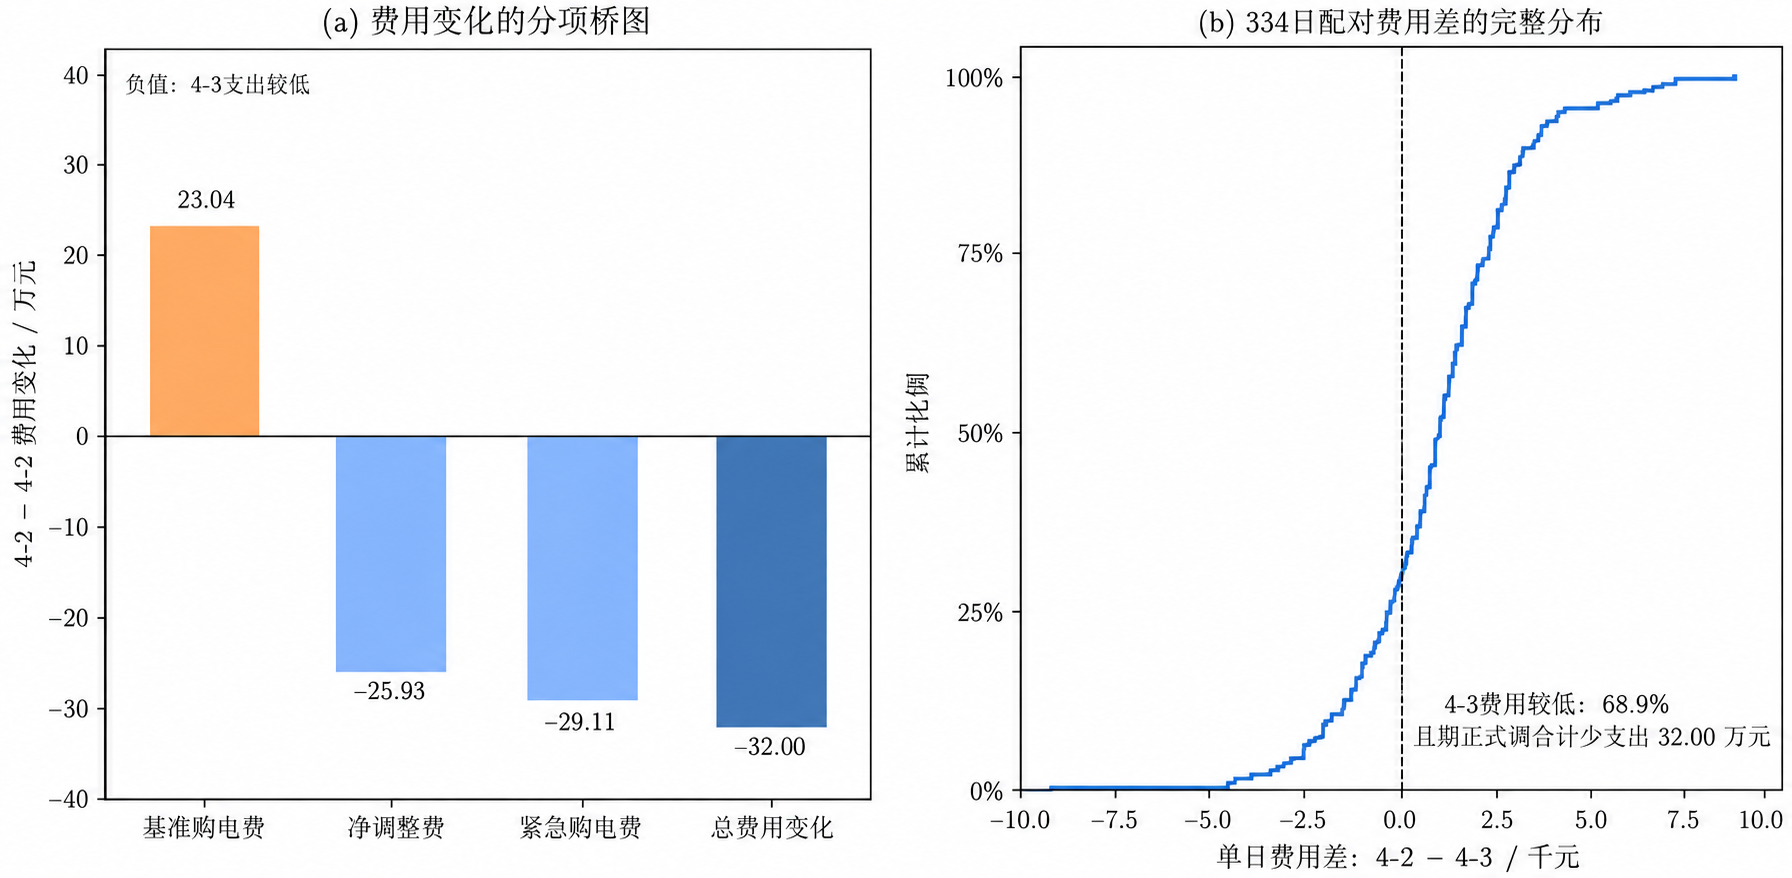
\includegraphics[width=0.96\textwidth]{figure/fig7_3_cost_change_bridge.png}
    \caption{四时点滚动调度的费用变化分解及逐日费用差分布}
    \label{fig:q4_cost_compare}
\end{figure}

由表~\ref{tab:q4_result}及图~\ref{fig:q4_cost_compare}(a)可见，
Q4-3 的基准购电费用较 Q4-2 增加 $23.04$ 万元，
但净调整费用和紧急购电费用分别减少 $25.93$ 万元和 $29.11$ 万元，
最终使全年总结算费用下降 $32.00$ 万元。
这表明滚动调度并非依靠压缩常规购电获得收益，而是通过日内信息更新及时修正
购电与储能决策，以适度增加事前供能保障换取更低的调整损失和高倍紧急补购风险。

图~\ref{fig:q4_cost_compare}(b)进一步表明，在 $334$ 个运行日中，
Q4-3 有 $230$ 日费用低于 Q4-2，占 $68.86\%$，
说明全年费用改善并非由少数极端日期驱动。
与此同时，紧急购电量和紧急购电费用分别下降 $33.30\%$ 和 $33.18\%$，
远高于总费用 $2.03\%$ 的降幅，说明四时点滚动更新的主要价值
在于降低供需偏差导致的高成本补购暴露。
\subsection{敏感性分析}

选取代表性工况，对 Wasserstein 半径及价格--净负荷联合距离权重进行单因素扰动，
结果见表~\ref{tab:q4_sensitivity}。

\begin{table}[H]
    \centering
    \caption{问题四关键参数敏感性分析}
    \label{tab:q4_sensitivity}
    \small
    \setlength{\tabcolsep}{5pt}
    \renewcommand{\arraystretch}{1.15}
    \begin{tabular}{llccc}
        \toprule
        模型 & 参数设置 & 参数含义 & 费用变化/\% & 紧急购电量变化/kWh \\
        \midrule

        \multirow{3}{*}{Q4-2}
        & $0.75\rho^*$ & 较弱鲁棒
        & $0.669\,[-0.113,\,1.530]$
        & $285.22\,[66.997,\,568.939]$ \\

        & $\rho^*$ & 基准设置
        & $0$
        & $0$ \\

        & $1.25\rho^*$ & 较强鲁棒
        & $-0.862\,[-2.173,\,0.212]$
        & $-308.58\,[-561.637,\,-41.385]$ \\
        \midrule

        \multirow{3}{*}{Q4-2}
        & $(0.7,\,0.3)$ & 净负荷权重较高
        & $-0.035\,[-1.489,\,1.194]$
        & $15.79\,[-382.110,\,458.974]$ \\

        & $(0.5,\,0.5)$ & 等权基准
        & $0$
        & $0$ \\

        & $(0.3,\,0.7)$ & 电价权重较高
        & $-1.228\,[-1.470,\,-0.215]$
        & $-260.48\,[-379.707,\,-47.503]$ \\
        \midrule

        \multirow{3}{*}{Q4-3}
        & $0.75\rho^*$ & 较弱鲁棒
        & $1.935\,[-0.152,\,4.022]$
        & $437.29\,[4.331,\,870.247]$ \\

        & $\rho^*$ & 基准设置
        & $0$
        & $0$ \\

        & $1.25\rho^*$ & 较强鲁棒
        & $-0.781\,[-1.808,\,0.246]$
        & $-225.44\,[-450.870,\,0]$ \\

        \bottomrule
    \end{tabular}
\end{table}
各扰动情形均保持最优可行，且能量平衡与储能运行约束均满足。
Q4-2 对关键参数变化总体较稳定；Q4-3 在常规工况下费用变化较小，
但高联合风险日最大变化达到 $4.02\%$，说明极端联合状态下滚动策略
对鲁棒参数更为敏感。

\section{模型评价}

\subsection{模型的优点}

\noindent 1) 本文按照“确定性调度--源荷不确定性调度--多时点滚动调整--价格与净负荷联合分布鲁棒调度”的递进结构建立统一模型，各问之间具有较强的继承性与解释性。

\noindent 2) 预测、场景构造与调度全过程严格遵守信息非前瞻原则，并利用样本外预测误差刻画不确定性，避免未来真实信息泄漏对策略评价造成偏差。

\noindent 3) 模型同时考虑能量平衡、储能状态转移、充放电功率及购电结算规则，并通过滚动时域与 Wasserstein 分布鲁棒优化兼顾经济性、物理可行性及极端场景风险。

\subsection{模型的缺点}

\noindent 1) 受题目数据与篇幅限制，模型未进一步考虑储能寿命衰减、自放电及线路损耗等长期运行因素，实际应用时需补充相应成本与物理参数。

\noindent 2) 源荷及电价不确定性主要依据有限历史样本外误差刻画，对历史中未出现的突发极端状态仍可能存在描述不足。





\CumcmAIUsed{代码调试和文献检索辅助}

% 参考文献
\begin{thebibliography}{99}

\bibitem{ke2017lightgbm}
KE G, MENG Q, FINLEY T, et al.
LightGBM: A highly efficient gradient boosting decision tree[C]//
Advances in Neural Information Processing Systems.
2017, 30: 3146--3154.

\bibitem{kaufman1990groups}
KAUFMAN L, ROUSSEEUW P J.
Finding Groups in Data: An Introduction to Cluster Analysis[M].
New York: John Wiley \& Sons, 1990.

\bibitem{dupacova2003scenario}
DUPAČOVÁ J, GRÖWE-KUSKA N, RÖMISCH W.
Scenario reduction in stochastic programming[J].
Mathematical Programming, 2003, 95(3): 493--511.
DOI:10.1007/s10107-002-0331-0.

\end{thebibliography}

\clearpage
\appendix
% 附录一级标题格式（仅作用于附录）
\titleformat{\section}
  {\centering\heiti\zihao{3}\bfseries}
  {附录~\thesection}
  {0.8em}
  {}
\section{支撑材料文件列表}
支撑材料位于 approval 目录，按下表列示。目录项包含该目录下的文件；完整逐文件清单见支撑材料中的文件清单。
\begin{longtable}{@{}p{0.07\textwidth}p{0.40\textwidth}p{0.43\textwidth}@{}}
\toprule
序号 & 文件路径 & 内容说明 \\
\midrule
\endhead
1 & src/q1/ & 问题一源程序及配套文件，共 17 份 \\
2 & src/q2/ & 问题二源程序及配套文件，共 42 份 \\
3 & src/q3/ & 问题三源程序及配套文件，共 35 份 \\
4 & src/q4/ & 问题四源程序及配套文件，共 20 份 \\
5 & src/sensitivity/ & 敏感性分析程序及配套文件，共 11 份 \\
6 & src/plots/ & 绘图与数据整理程序及配套文件，共 26 份 \\
7 & src/问题1/ & 问题一补充程序及配套文件，共 1 份 \\
8 & docs/ & 题目资料、模型文档与运行依据 \\
9 & inputs/ & 程序所需输入与价格缓存 \\
10 & outputs/ & 计算结果、冻结预测及实验数据 \\
11 & 参考文献/ & 三项参考文献书目、两篇论文全文及获取说明 \\
12 & README.md & 支撑材料总说明 \\
13 & 运行说明.md & 程序入口与运行步骤 \\
14 & AI使用报告.md & AI 辅助使用情况说明 \\
15 & 文件清单.csv & 支撑材料逐文件清单 \\
16 & 校验结果.json & 支撑材料已有校验记录 \\
\bottomrule
\end{longtable}

\section{完整源程序}
本附录收录支撑材料 src 目录中的全部 145 份源程序文件，按问题及用途分组，保留完整程序内容。论文工程中的对应副本位于 code/src 目录；依赖说明和配套数据文件随源码一并保存。
\lstset{basicstyle=\cumcmcodefont\scriptsize,breaklines=true,breakatwhitespace=false,columns=fullflexible,keepspaces=true,showstringspaces=false,tabsize=4}

\subsection{问题一源程序}
\subsubsection*{src/q1/analysis.py}
\lstinputlisting[language=Python]{code/src/q1/analysis.py}

\subsubsection*{src/q1/analysis\_report.py}
\lstinputlisting[language=Python]{code/src/q1/analysis_report.py}

\subsubsection*{src/q1/device\_sensitivity.py}
\lstinputlisting[language=Python]{code/src/q1/device_sensitivity.py}

\subsubsection*{src/q1/export.py}
\lstinputlisting[language=Python]{code/src/q1/export.py}

\subsubsection*{src/q1/export\_submission.mjs}
\lstinputlisting[language={}]{code/src/q1/export_submission.mjs}

\subsubsection*{src/q1/model.py}
\lstinputlisting[language=Python]{code/src/q1/model.py}

\subsubsection*{src/q1/pipeline.py}
\lstinputlisting[language=Python]{code/src/q1/pipeline.py}

\subsubsection*{src/q1/prepare\_paper\_materials.py}
\lstinputlisting[language=Python]{code/src/q1/prepare_paper_materials.py}

\subsubsection*{src/q1/report.py}
\lstinputlisting[language=Python]{code/src/q1/report.py}

\subsubsection*{src/q1/review\_compact\_q1.py}
\lstinputlisting[language=Python]{code/src/q1/review_compact_q1.py}

\subsubsection*{src/q1/run.py}
\lstinputlisting[language=Python]{code/src/q1/run.py}

\subsubsection*{src/q1/test\_analysis.py}
\lstinputlisting[language=Python]{code/src/q1/test_analysis.py}

\subsubsection*{src/q1/test\_q1.py}
\lstinputlisting[language=Python]{code/src/q1/test_q1.py}

\subsubsection*{src/q1/test\_review.py}
\lstinputlisting[language=Python]{code/src/q1/test_review.py}

\subsubsection*{src/q1/traceability.py}
\lstinputlisting[language=Python]{code/src/q1/traceability.py}

\subsection{问题二源程序}
\subsubsection*{src/q2/backtest.py}
\lstinputlisting[language=Python]{code/src/q2/backtest.py}

\subsubsection*{src/q2/baseline\_reuse.py}
\lstinputlisting[language=Python]{code/src/q2/baseline_reuse.py}

\subsubsection*{src/q2/benchmarks/horizon\_for\_figure.py}
\lstinputlisting[language=Python]{code/src/q2/benchmarks/horizon_for_figure.py}

\subsubsection*{src/q2/benchmarks/precision\_pair.py}
\lstinputlisting[language=Python]{code/src/q2/benchmarks/precision_pair.py}

\subsubsection*{src/q2/benchmarks/precision\_pair\_report.py}
\lstinputlisting[language=Python]{code/src/q2/benchmarks/precision_pair_report.py}

\subsubsection*{src/q2/benchmarks/precision\_sweep.py}
\lstinputlisting[language=Python]{code/src/q2/benchmarks/precision_sweep.py}

\subsubsection*{src/q2/checkpoint.py}
\lstinputlisting[language=Python]{code/src/q2/checkpoint.py}

\subsubsection*{src/q2/comparators.py}
\lstinputlisting[language=Python]{code/src/q2/comparators.py}

\subsubsection*{src/q2/data.py}
\lstinputlisting[language=Python]{code/src/q2/data.py}

\subsubsection*{src/q2/deliverables/export\_partial.py}
\lstinputlisting[language=Python]{code/src/q2/deliverables/export_partial.py}

\subsubsection*{src/q2/diagnostics.py}
\lstinputlisting[language=Python]{code/src/q2/diagnostics.py}

\subsubsection*{src/q2/dispatch.py}
\lstinputlisting[language=Python]{code/src/q2/dispatch.py}

\subsubsection*{src/q2/execution.py}
\lstinputlisting[language=Python]{code/src/q2/execution.py}

\subsubsection*{src/q2/experiments.py}
\lstinputlisting[language=Python]{code/src/q2/experiments.py}

\subsubsection*{src/q2/export\_dispatch.py}
\lstinputlisting[language=Python]{code/src/q2/export_dispatch.py}

\subsubsection*{src/q2/figures.py}
\lstinputlisting[language=Python]{code/src/q2/figures.py}

\subsubsection*{src/q2/final\_diagnostics.py}
\lstinputlisting[language=Python]{code/src/q2/final_diagnostics.py}

\subsubsection*{src/q2/final\_report.py}
\lstinputlisting[language=Python]{code/src/q2/final_report.py}

\subsubsection*{src/q2/final\_traceability.py}
\lstinputlisting[language=Python]{code/src/q2/final_traceability.py}

\subsubsection*{src/q2/forecast.py}
\lstinputlisting[language=Python]{code/src/q2/forecast.py}

\subsubsection*{src/q2/full\_run.py}
\lstinputlisting[language=Python]{code/src/q2/full_run.py}

\subsubsection*{src/q2/incumbent.py}
\lstinputlisting[language=Python]{code/src/q2/incumbent.py}

\subsubsection*{src/q2/linear\_policy.py}
\lstinputlisting[language=Python]{code/src/q2/linear_policy.py}

\subsubsection*{src/q2/optimization.py}
\lstinputlisting[language=Python]{code/src/q2/optimization.py}

\subsubsection*{src/q2/policy.py}
\lstinputlisting[language=Python]{code/src/q2/policy.py}

\subsubsection*{src/q2/protocol.py}
\lstinputlisting[language=Python]{code/src/q2/protocol.py}

\subsubsection*{src/q2/relaxation.py}
\lstinputlisting[language=Python]{code/src/q2/relaxation.py}

\subsubsection*{src/q2/report.py}
\lstinputlisting[language=Python]{code/src/q2/report.py}

\subsubsection*{src/q2/rolling.py}
\lstinputlisting[language=Python]{code/src/q2/rolling.py}

\subsubsection*{src/q2/run.py}
\lstinputlisting[language=Python]{code/src/q2/run.py}

\subsubsection*{src/q2/scenarios.py}
\lstinputlisting[language=Python]{code/src/q2/scenarios.py}

\subsubsection*{src/q2/shadows.py}
\lstinputlisting[language=Python]{code/src/q2/shadows.py}

\subsubsection*{src/q2/test\_baseline\_reuse.py}
\lstinputlisting[language=Python]{code/src/q2/test_baseline_reuse.py}

\subsubsection*{src/q2/test\_dispatch.py}
\lstinputlisting[language=Python]{code/src/q2/test_dispatch.py}

\subsubsection*{src/q2/test\_execution.py}
\lstinputlisting[language=Python]{code/src/q2/test_execution.py}

\subsubsection*{src/q2/test\_forecast\_dispatch.py}
\lstinputlisting[language=Python]{code/src/q2/test_forecast_dispatch.py}

\subsubsection*{src/q2/test\_full\_run.py}
\lstinputlisting[language=Python]{code/src/q2/test_full_run.py}

\subsubsection*{src/q2/test\_horizon\_execution.py}
\lstinputlisting[language=Python]{code/src/q2/test_horizon_execution.py}

\subsubsection*{src/q2/test\_linear\_policy.py}
\lstinputlisting[language=Python]{code/src/q2/test_linear_policy.py}

\subsubsection*{src/q2/test\_q2.py}
\lstinputlisting[language=Python]{code/src/q2/test_q2.py}

\subsubsection*{src/q2/traceability.py}
\lstinputlisting[language=Python]{code/src/q2/traceability.py}

\subsection{问题三源程序}
\subsubsection*{src/q3/\_\_init\_\_.py}
\lstinputlisting[language=Python]{code/src/q3/__init__.py}

\subsubsection*{src/q3/analysis.py}
\lstinputlisting[language=Python]{code/src/q3/analysis.py}

\subsubsection*{src/q3/checkpoint.py}
\lstinputlisting[language=Python]{code/src/q3/checkpoint.py}

\subsubsection*{src/q3/config.py}
\lstinputlisting[language=Python]{code/src/q3/config.py}

\subsubsection*{src/q3/data.py}
\lstinputlisting[language=Python]{code/src/q3/data.py}

\subsubsection*{src/q3/export.py}
\lstinputlisting[language=Python]{code/src/q3/export.py}

\subsubsection*{src/q3/fast\_solver.py}
\lstinputlisting[language=Python]{code/src/q3/fast_solver.py}

\subsubsection*{src/q3/full\_run.py}
\lstinputlisting[language=Python]{code/src/q3/full_run.py}

\subsubsection*{src/q3/gurobi\_backend.py}
\lstinputlisting[language=Python]{code/src/q3/gurobi_backend.py}

\subsubsection*{src/q3/incumbent.py}
\lstinputlisting[language=Python]{code/src/q3/incumbent.py}

\subsubsection*{src/q3/migrate\_rescue.py}
\lstinputlisting[language=Python]{code/src/q3/migrate_rescue.py}

\subsubsection*{src/q3/migrate\_solver.py}
\lstinputlisting[language=Python]{code/src/q3/migrate_solver.py}

\subsubsection*{src/q3/multistage.py}
\lstinputlisting[language=Python]{code/src/q3/multistage.py}

\subsubsection*{src/q3/optimization.py}
\lstinputlisting[language=Python]{code/src/q3/optimization.py}

\subsubsection*{src/q3/parallel.py}
\lstinputlisting[language=Python]{code/src/q3/parallel.py}

\subsubsection*{src/q3/parallel\_benchmark.py}
\lstinputlisting[language=Python]{code/src/q3/parallel_benchmark.py}

\subsubsection*{src/q3/physics.py}
\lstinputlisting[language=Python]{code/src/q3/physics.py}

\subsubsection*{src/q3/rolling.py}
\lstinputlisting[language=Python]{code/src/q3/rolling.py}

\subsubsection*{src/q3/run.py}
\lstinputlisting[language=Python]{code/src/q3/run.py}

\subsubsection*{src/q3/sampled.py}
\lstinputlisting[language=Python]{code/src/q3/sampled.py}

\subsubsection*{src/q3/scenarios.py}
\lstinputlisting[language=Python]{code/src/q3/scenarios.py}

\subsubsection*{src/q3/solver\_probe.py}
\lstinputlisting[language=Python]{code/src/q3/solver_probe.py}

\subsubsection*{src/q3/status\_server.py}
\lstinputlisting[language=Python]{code/src/q3/status_server.py}

\subsubsection*{src/q3/terminal.py}
\lstinputlisting[language=Python]{code/src/q3/terminal.py}

\subsubsection*{src/q3/test\_fast\_solver.py}
\lstinputlisting[language=Python]{code/src/q3/test_fast_solver.py}

\subsubsection*{src/q3/test\_full\_run.py}
\lstinputlisting[language=Python]{code/src/q3/test_full_run.py}

\subsubsection*{src/q3/test\_gurobi\_backend.py}
\lstinputlisting[language=Python]{code/src/q3/test_gurobi_backend.py}

\subsubsection*{src/q3/test\_parallel.py}
\lstinputlisting[language=Python]{code/src/q3/test_parallel.py}

\subsubsection*{src/q3/test\_production\_rescue.py}
\lstinputlisting[language=Python]{code/src/q3/test_production_rescue.py}

\subsubsection*{src/q3/test\_q3.py}
\lstinputlisting[language=Python]{code/src/q3/test_q3.py}

\subsubsection*{src/q3/test\_solver\_acceleration.py}
\lstinputlisting[language=Python]{code/src/q3/test_solver_acceleration.py}

\subsubsection*{src/q3/test\_validation.py}
\lstinputlisting[language=Python]{code/src/q3/test_validation.py}

\subsubsection*{src/q3/traceability.py}
\lstinputlisting[language=Python]{code/src/q3/traceability.py}

\subsubsection*{src/q3/validation.py}
\lstinputlisting[language=Python]{code/src/q3/validation.py}

\subsection{问题四源程序}
\subsubsection*{src/q4/\_\_init\_\_.py}
\lstinputlisting[language=Python]{code/src/q4/__init__.py}

\subsubsection*{src/q4/config.py}
\lstinputlisting[language=Python]{code/src/q4/config.py}

\subsubsection*{src/q4/data.py}
\lstinputlisting[language=Python]{code/src/q4/data.py}

\subsubsection*{src/q4/diagnostics.py}
\lstinputlisting[language=Python]{code/src/q4/diagnostics.py}

\subsubsection*{src/q4/export.py}
\lstinputlisting[language=Python]{code/src/q4/export.py}

\subsubsection*{src/q4/optimization.py}
\lstinputlisting[language=Python]{code/src/q4/optimization.py}

\subsubsection*{src/q4/physics.py}
\lstinputlisting[language=Python]{code/src/q4/physics.py}

\subsubsection*{src/q4/price.py}
\lstinputlisting[language=Python]{code/src/q4/price.py}

\subsubsection*{src/q4/rescue/check\_apr18.py}
\lstinputlisting[language=Python]{code/src/q4/rescue/check_apr18.py}

\subsubsection*{src/q4/rescue/launch\_full.py}
\lstinputlisting[language=Python]{code/src/q4/rescue/launch_full.py}

\subsubsection*{src/q4/rescue/launch\_q43\_v3.py}
\lstinputlisting[language=Python]{code/src/q4/rescue/launch_q43_v3.py}

\subsubsection*{src/q4/rescue/verify\_full.py}
\lstinputlisting[language=Python]{code/src/q4/rescue/verify_full.py}

\subsubsection*{src/q4/rolling.py}
\lstinputlisting[language=Python]{code/src/q4/rolling.py}

\subsubsection*{src/q4/run.py}
\lstinputlisting[language=Python]{code/src/q4/run.py}

\subsubsection*{src/q4/scenarios.py}
\lstinputlisting[language=Python]{code/src/q4/scenarios.py}

\subsubsection*{src/q4/test\_q4.py}
\lstinputlisting[language=Python]{code/src/q4/test_q4.py}

\subsubsection*{src/q4/test\_rescue.py}
\lstinputlisting[language=Python]{code/src/q4/test_rescue.py}

\subsubsection*{src/q4/traceability.py}
\lstinputlisting[language=Python]{code/src/q4/traceability.py}

\subsubsection*{src/q4/vertical\_slice.py}
\lstinputlisting[language=Python]{code/src/q4/vertical_slice.py}

\subsection{敏感性分析程序}
\subsubsection*{src/sensitivity/common.py}
\lstinputlisting[language=Python]{code/src/sensitivity/common.py}

\subsubsection*{src/sensitivity/prepare.py}
\lstinputlisting[language=Python]{code/src/sensitivity/prepare.py}

\subsubsection*{src/sensitivity/q2.py}
\lstinputlisting[language=Python]{code/src/sensitivity/q2.py}

\subsubsection*{src/sensitivity/q3.py}
\lstinputlisting[language=Python]{code/src/sensitivity/q3.py}

\subsubsection*{src/sensitivity/q4\_experiment.py}
\lstinputlisting[language=Python]{code/src/sensitivity/q4_experiment.py}

\subsubsection*{src/sensitivity/q4\_report.py}
\lstinputlisting[language=Python]{code/src/sensitivity/q4_report.py}

\subsubsection*{src/sensitivity/report.py}
\lstinputlisting[language=Python]{code/src/sensitivity/report.py}

\subsubsection*{src/sensitivity/run.py}
\lstinputlisting[language=Python]{code/src/sensitivity/run.py}

\subsubsection*{src/sensitivity/status\_server.py}
\lstinputlisting[language=Python]{code/src/sensitivity/status_server.py}

\subsubsection*{src/sensitivity/test\_sensitivity.py}
\lstinputlisting[language=Python]{code/src/sensitivity/test_sensitivity.py}

\subsubsection*{src/sensitivity/verify.py}
\lstinputlisting[language=Python]{code/src/sensitivity/verify.py}

\subsection{绘图与数据整理程序}
\subsubsection*{src/plots/catalog.py}
\lstinputlisting[language=Python]{code/src/plots/catalog.py}

\subsubsection*{src/plots/common.py}
\lstinputlisting[language=Python]{code/src/plots/common.py}

\subsubsection*{src/plots/project\_expansion.py}
\lstinputlisting[language=Python]{code/src/plots/project_expansion.py}

\subsubsection*{src/plots/project\_expansion\_data.py}
\lstinputlisting[language=Python]{code/src/plots/project_expansion_data.py}

\subsubsection*{src/plots/q1\_legacy.py}
\lstinputlisting[language=Python]{code/src/plots/q1_legacy.py}

\subsubsection*{src/plots/q1\_paper.py}
\lstinputlisting[language=Python]{code/src/plots/q1_paper.py}

\subsubsection*{src/plots/q2.py}
\lstinputlisting[language=Python]{code/src/plots/q2.py}

\subsubsection*{src/plots/q2\_dispatch.py}
\lstinputlisting[language=Python]{code/src/plots/q2_dispatch.py}

\subsubsection*{src/plots/q2\_paper\_data.py}
\lstinputlisting[language=Python]{code/src/plots/q2_paper_data.py}

\subsubsection*{src/plots/q2\_paper\_final.py}
\lstinputlisting[language=Python]{code/src/plots/q2_paper_final.py}

\subsubsection*{src/plots/q2\_paper\_verify.py}
\lstinputlisting[language=Python]{code/src/plots/q2_paper_verify.py}

\subsubsection*{src/plots/q3.py}
\lstinputlisting[language=Python]{code/src/plots/q3.py}

\subsubsection*{src/plots/q3\_paper\_core.py}
\lstinputlisting[language=Python]{code/src/plots/q3_paper_core.py}

\subsubsection*{src/plots/q3\_paper\_data.py}
\lstinputlisting[language=Python]{code/src/plots/q3_paper_data.py}

\subsubsection*{src/plots/q3\_paper\_final.py}
\lstinputlisting[language=Python]{code/src/plots/q3_paper_final.py}

\subsubsection*{src/plots/q3\_paper\_package.py}
\lstinputlisting[language=Python]{code/src/plots/q3_paper_package.py}

\subsubsection*{src/plots/q3\_paper\_verify.py}
\lstinputlisting[language=Python]{code/src/plots/q3_paper_verify.py}

\subsubsection*{src/plots/q4\_paper\_data.py}
\lstinputlisting[language=Python]{code/src/plots/q4_paper_data.py}

\subsubsection*{src/plots/q4\_paper\_final.py}
\lstinputlisting[language=Python]{code/src/plots/q4_paper_final.py}

\subsubsection*{src/plots/q4\_paper\_package.py}
\lstinputlisting[language=Python]{code/src/plots/q4_paper_package.py}

\subsubsection*{src/plots/q4\_paper\_verify.py}
\lstinputlisting[language=Python]{code/src/plots/q4_paper_verify.py}

\subsubsection*{src/plots/replot\_existing.py}
\lstinputlisting[language=Python]{code/src/plots/replot_existing.py}

\subsubsection*{src/plots/run.py}
\lstinputlisting[language=Python]{code/src/plots/run.py}

\subsubsection*{src/plots/verify.py}
\lstinputlisting[language=Python]{code/src/plots/verify.py}

\subsection{问题一补充程序}
\subsubsection*{src/问题1/review\_temporary\_plan.py}
\lstinputlisting[language=Python]{code/src/问题1/review_temporary_plan.py}

\end{document}
